\documentclass[twoside,paper=a4,fontsize=11pt]{report}

%*******************************************************
% From page 7 of Preparing and Submitting Your
% Thesis - A guide for MPhil and PhD students:
% The thesis submitted for examination shall be typewritten
% or printed on one side or both sides of International size
% A4 paper (except for drawings, maps or tables on
% which no restriction is placed), with a margin of
% not less than 35mm on both right and left-hand
% edges of each page.
% There is no stipulation for the top and bottom margins,
% but it is recommended that they should be 25mm.
% From page10:
% Font heights are usually measured in points and
% the most easily readable fonts are 10 point and 12 point.
%*******************************************************

\usepackage[left=37mm,right=37mm,top=27mm,bottom=27mm]{geometry}

%*******************************************************
% Include packages that you wish to use.
%*******************************************************

\usepackage{tikz}
\usetikzlibrary{shapes,arrows}

\usepackage{lipsum} % this generates dummy text

\usepackage{multicol} % use multicolumn
\usepackage{rotating} % to create a figure in landscape mode

\usepackage{natbib} % this is for bibliography
\usepackage{setspace} % this is for setting line spacing

\usepackage{longtable} % this is for longtable


\usepackage{array}


\usepackage{amsthm}
\usepackage{amsmath}
\usepackage{calc}
\usepackage{float}
\usepackage{graphicx}
\usepackage{setspace}
\usepackage{url}

\usepackage{nomencl}
\makenomenclature

%*******************************************************
% Define hyphenation for some special words
%*******************************************************

\usepackage{hyphenat} % this define hyphenation, an example is given in the next four lines.
\hyphenation{pro-ban-da}
\hyphenation{pro-ban-dum}
\hyphenation{pen-ul-ti-mate}
\hyphenation{sche-ma-tic}

%*******************************************************
% Make "clickable" Table of Contents
%*******************************************************
\usepackage{color}   %May be necessary if you want to color links
\usepackage{hyperref}
\hypersetup{
    colorlinks=true, %set true if you want colored links
    linktoc=all,         %set to all if you want both sections and subsections linked
    linkcolor=blue,  %choose some color, e.g. blue, if you want links to stand out
    }

%*******************************************************
% This is the start of the thesis
%*******************************************************

\begin{document}

\linespread{1.2} % change it to 1 becomes single line spacing. Change it to 1.5 is a half line spacing.

%*******************************************************
% From page 10 of Preparing and Submitting Your Thesis
% A guide for MPhil and PhD students:
% Modern word processing programs will automatically
% adjust the line spacing to match the size of text on any line.
% Single line spacing will produce a dense but readable
% text: the text may seem less formidable if one and a
% spacing is used. Double spacing results in a rather
% empty looking page and significantly increases
% the number of pages in a thesis.
%*******************************************************

%*******************************************************
% These are front matters.
% Abstract
% Title page
% Dedication
% Declaration
% Acknowledgment
% Publication (Optional)
% Table of Contents (Including List of Tables and List of Figures)
%*******************************************************

%*******************************************************
% Abstract
%*******************************************************
\phantomsection
\addcontentsline{toc}{chapter}{Abstract}

\begin{center}

Abstract of thesis entitled\\

\bigskip

    \huge\textbf{Search for chargino and neutralino production in final states with two same-sign leptons, jets and missing transverse momentum at $\sqrt{s} = 13$ TeV with the ATLAS detector} \\

    \bigskip

    {\normalsize Submitted by}\\

\bigskip

    \Large{\textbf{Cheuk Yee LO}}\\

\bigskip

{\normalsize
for the degree of Doctor of Philosophy\\
at The University of Hong Kong\\
in November 2018\\}

\end{center}

\bigskip

The Standard Model in particle physics has successfully explained almost all experimental results in the microscopic scale with high accuracy.
However, the nature of the dark matter and the hierarchy problem of Higgs mass are still the unanswered questions.
Supersymmetry (SUSY) is one of the most promising theories beyond the Standard Model, that might answer these questions.
In the recent searches for supersymmetric particles that are involved in strong interaction, their masses are above 1 TeV.
This might suggest that the pair production of electroweak gauginos is a dominant SUSY production process at the Large Hadron Collider (LHC).
Also, the recent upgrade that the center-of-mass energy of the proton-proton collisions $\sqrt{s}$ has increased to 13 TeV, opened a new phase of exploration for SUSY.
% word count: 122

In this thesis, a search is presented for the electroweak pair production of a chargino and a neutralino ($p + p \rightarrow \tilde{\chi}_1^\pm + \tilde{\chi}_2^0$),
where the chargino decays to the lightest neutralino and a W boson ($\tilde{\chi}_1^\pm \rightarrow \tilde{\chi}_1^0 + W$),
and the neutralino decays to the lightest neutralino and a Standard Model like Higgs boson with mass 125 GeV ($\tilde{\chi}_2^0 \rightarrow \tilde{\chi}_1^0 + h$).
The final state with two same-sign leptons, jets and missing transverse momentum are considered in this search.
The two leptons come from the leptonically decay of the W boson and the Higgs boson with the decay modes of  $h \rightarrow WW$, $h \rightarrow \tau \tau$ or $h \rightarrow ZZ$.
This analysis is based on the proton-proton collision data delivered by the LHC at $\sqrt{s}$ = 13 TeV with the ATLAS detector.
The integrated luminosity of data is 36.1 fb$^{-1}$.
% word count: 119

%The results of this analysis are combined with the results of the search for final state with 3 leptons.
The exclusion limit for the masses of $\tilde{\chi}_1^\pm$ and $\tilde{\chi}_2^0$ is extended up to 245 GeV, while the exclusion limit for the mass of $\tilde{\chi}_1^0$ is extended up to 40 GeV, with 95\% confidence level, in the context of a simplified supersymmetric model.
% word count: 43

\bigskip

\begin{center}

\rule{6cm}{0.025cm}\\
{\slshape An abstract of exactly 284 words}

\end{center}


%*******************************************************
% Titlepage
%*******************************************************
\phantomsection
\addcontentsline{toc}{chapter}{Title Page}

\begin{center}
    \large
        \hfill
        \vfill
    \begingroup
        \huge\textsc{\textbf{This is the title of my thesis}} \\
        \bigskip
    \endgroup
    by\\
    \bigskip
    \Large\textsc{\textbf{Cheuk Yee LO}}\\
    \vfill
    \vfill
    \vfill
{\normalsize
A thesis submitted in partial fulfilment of the requirements for\\
the Degree of Doctor of Philosophy\\
at The University of Hong Kong.\\
    \bigskip
August 2018}
    \vfill
\end{center}


\cleardoublepage

\pagenumbering{roman}

\pagestyle{plain}



%*******************************************************
% This program is free software: you can redistribute it and/or modify
% it under the terms of the GNU General Public License as published by
% the Free Software Foundation, either version 3 of the License, or
% (at your option) any later version.
%
% This program is distributed in the hope that it will be useful,
% but WITHOUT ANY WARRANTY; without even the implied warranty of
% MERCHANTABILITY or FITNESS FOR A PARTICULAR PURPOSE.  See the
% GNU General Public License for more details.
%
% You should have received a copy of the GNU General Public License
% along with this program.  If not, see <http://www.gnu.org/licenses/>.
%*******************************************************
% Declaration
%*******************************************************

\addcontentsline{toc}{chapter}{Declaration}%% to be removed

\chapter*{Declarations}

I declare that this thesis represents my own work, except where due acknowledgement is made, and that it has not been previously included in a thesis, dissertation or report submitted to this University or to any other institution for a degree, diploma or other qualifications.% This is copied from the declaration statement from the Handbook.

\bigskip
\bigskip
\bigskip
\bigskip
\bigskip
\bigskip
\bigskip
\bigskip

\begin{flushright}
    \begin{tabular}{p{1cm} p{4cm}}
        Signed & \dotfill \\
           & \center Yufen CHUN\\
    \end{tabular}
\end{flushright}

\bigskip
\bigskip
\bigskip


\cleardoublepage
%*******************************************************
% Acknowledgments
%*******************************************************

\addcontentsline{toc}{chapter}{Acknowledgments}
\chapter*{Acknowledgments}

I would like to thank my supervisor Tu Yanjun for giving me the opportunity to do the research, for her support on my research and for her guidance and suggestions on my analysis.

I would like to thank Zhang Dongliang. He taught me almost everything on the analysis, including linux shell, ROOT, vim, svn, RootCore, dq2, rucio, grid, panda, latex, trigger system, GRL, and more.
He also help our group to write the multiLepSearch package to generate the ntuple.

I would like to thank Daniela Paredes, the postdoc in our group.
She gave a lot of suggestions on my analysis.
She also help our group to do analysis.



\cleardoublepage
%*******************************************************
% Table of Contents
%*******************************************************

\phantomsection
\addcontentsline{toc}{chapter}{Contents}

\setcounter{tocdepth}{2} % <-- 2 includes up to subsections in the ToC
\setcounter{secnumdepth}{3} % <-- 3 numbers up to subsubsections

\tableofcontents 

%*******************************************************
% List of Figures and of the Tables
%*******************************************************

\clearpage
\phantomsection
\addcontentsline{toc}{chapter}{List of Figures}
\listoffigures

\clearpage
\phantomsection
\addcontentsline{toc}{chapter}{List of Tables}
\listoftables


\cleardoublepage
\clearpage
\phantomsection
\addcontentsline{toc}{chapter}{List of Abbreviations and Symbols}

\nomenclature{CERN}{the European Organization for Nuclear Research}
\nomenclature{SM}{Standard Model}
\nomenclature{BSM}{beyond the Standard Model}
\nomenclature{SUSY}{Supersymmetry}
\nomenclature{LHC}{Large Hadron Collider}
\nomenclature{lepton}{refer to electron or muon}
\nomenclature{jet}{a particle shower in a narrow cone from the hadronization of a quark or a gluon}

\nomenclature{MC}{Monte Carlo Simulation}
\nomenclature{Data}{the experimental data}
\nomenclature{BG}{background}

\nomenclature{SR}{signal region}
\nomenclature{CR}{control region}
\nomenclature{VR}{validation region}

\nomenclature{N-1 plot}{The plot with all selections are applied, except the selection for that variable}
\nomenclature{yield}{The resulting number of events}

\nomenclature{SS}{same sign}
\nomenclature{OS}{opposite sign}

\nomenclature{$p_T$}{transverse momentum}
\nomenclature{$\eta$}{pseudorapidity}
\nomenclature{MET}{missing transverse energy}
\nomenclature{cut}{selection cut}

\renewcommand{\nomname}{List of Abbreviations and Symbols}
\printnomenclature

\renewcommand{\nomname}{List of Abbreviations and Symbols}
\printnomenclature

%*******************************************************
% Mainmatter
%*******************************************************

\pagenumbering{arabic}

\cleardoublepage

%************************************************
\chapter{This is chapter one}
\label{ch:name4}
%************************************************
\section{Introduction}
\label{sec:ch_4_introduction}

\citet{Berg2016} argues that this is a topic sentence followed by explanation, elaboration and examples to introduce the next three subsections. The last sentence of this paragraph shall introduce the next paragraph.

This is a topic sentence followed by explanation, elaboration and examples to introduce the next three subsections \citep{Collins2016}. The last sentence of this paragraph shall introduce the next paragraph.

\citet{Graham2016} and \citet{Grant2016} assert that this is a topic sentence followed by explanation, elaboration and examples to introduce the next three subsections. The last sentence of this paragraph shall introduce the next paragraph.

\section{First main stuff}
\label{sec:ch_4_firstmain}

This is a topic sentence followed by explanation, elaboration and examples to introduce this paragraph \citep{Haney2016}. The last sentence of this paragraph shall introduce the next paragraph.

This is a topic sentence followed by explanation, elaboration and examples to introduce this paragraph \citep{Jordan2016,Morgan2016}. The last sentence of this paragraph shall introduce the next paragraph.

This is a topic sentence followed by explanation, elaboration and examples to introduce this paragraph. The last sentence of this paragraph shall introduce the next paragraph.

\section{Second main stuff}
\label{sec:ch_4_secondmain}

This is a topic sentence followed by explanation, elaboration and examples to introduce this paragraph \citep{Scott2016}. The last sentence of this paragraph shall introduce the next paragraph.
 
As \citet{Wells2016} and \citet{Williamson2016}.
This is a topic sentence followed by explanation, elaboration and examples to introduce this paragraph \citep{Stewart2016}. The last sentence of this paragraph shall introduce the next paragraph.

This is a topic sentence followed by explanation, elaboration and examples to introduce this paragraph \citep{Gallagher2016}. The last sentence of this paragraph shall introduce the next paragraph.


\cleardoublepage

%************************************************
\chapter{Literature review}
\label{ch:name2}
%************************************************

\section{Introduction}
\label{sec:ch_2_introduction}

This is a topic sentence followed by explanation, elaboration and examples to introduce the next three subsections. The last sentence of this paragraph shall introduce the next paragraph.

\section{First main stuff}
\label{sec:ch_2_firstmain}

This is a topic sentence followed by explanation, elaboration and examples to introduce this paragraph. The last sentence of this paragraph shall introduce the next paragraph.


\cleardoublepage



%*******************************************************
% This program is free software: you can redistribute it and/or modify
% it under the terms of the GNU General Public License as published by
% the Free Software Foundation, either version 3 of the License, or
% (at your option) any later version.
%
% This program is distributed in the hope that it will be useful,
% but WITHOUT ANY WARRANTY; without even the implied warranty of
% MERCHANTABILITY or FITNESS FOR A PARTICULAR PURPOSE.  See the
% GNU General Public License for more details.
%
% You should have received a copy of the GNU General Public License
% along with this program.  If not, see <http://www.gnu.org/licenses/>.
%************************************************
\chapter{This is chapter three}
\label{ch:name3}
%************************************************

\begin{flushright}
{\slshape Lorem ipsum dolor sit amet, consectetuer adipiscing.}\\
{\slshape Aenean commodo ligula eget dolor. Aenean massa.}\\
% This generate dummy text. Remove this line and replace by your quote.
\medskip
--- John Doe,\\
Unified Theory of the Important Theories,\\
{\slshape An Important Journal},\\
Vol.~123, pp.~1234--1243, Dec.~2016.\\
\end{flushright}

\bigskip

\section{Introduction}
\label{sec:ch_3_introduction}

This is a topic sentence followed by explanation, elaboration and examples to introduce the next three subsections. The last sentence of this paragraph shall introduce the next paragraph. \lipsum[1]

This is a topic sentence followed by explanation, elaboration and examples to introduce the next three subsections. The last sentence of this paragraph shall introduce the next paragraph. \lipsum[1]

This is a topic sentence followed by explanation, elaboration and examples to introduce the next three subsections. The last sentence of this paragraph shall introduce the next paragraph. \lipsum[1]

\section{First main stuff}
\label{sec:ch_3_firstmain}

This is a topic sentence followed by explanation, elaboration and examples to introduce this paragraph. The last sentence of this paragraph shall introduce the next paragraph. \lipsum[1]

This is a topic sentence followed by explanation, elaboration and examples to introduce this paragraph. The last sentence of this paragraph shall introduce the next paragraph. \lipsum[1]

Table \ref{table:1} is an example of the observations.

\begin{table}[h!]
\centering
 \begin{tabular}{||c c c c||} 
 \hline
 Col1 & Col2 & Col2 & Col3 \\ [0.5ex] 
 \hline\hline
 1 & 161 & 8787 & 7887 \\ 
 2 & 272 & 6767 & 5445 \\
 3 & 545 & 7878 & 7557 \\
 4 & 545 & 1717 & 7007 \\
 5 & 888 & 7887 & 6363 \\ [1ex] 
 \hline
 \end{tabular}
 \caption{Table to prove captions and labels}
 \label{table:1}
\end{table}

This is a topic sentence followed by explanation, elaboration and examples to introduce this paragraph. The last sentence of this paragraph shall introduce the next paragraph. \lipsum[1]

\section{Second main stuff}
\label{sec:ch_3_secondmain}


This is a topic sentence followed by explanation, elaboration and examples to introduce this paragraph. The last sentence of this paragraph shall introduce the next paragraph. \lipsum[1]

This is a topic sentence followed by explanation, elaboration and examples to introduce this paragraph. The last sentence of this paragraph shall introduce the next paragraph. \lipsum[1]

This is a topic sentence followed by explanation, elaboration and examples to introduce this paragraph. The last sentence of this paragraph shall introduce the next paragraph. \lipsum[1]

\section{Third main stuff}
\label{sec:ch_3_thirdmain}

This is a topic sentence followed by explanation, elaboration and examples to introduce this paragraph. The last sentence of this paragraph shall introduce the next paragraph. \lipsum[1]

This is a topic sentence followed by explanation, elaboration and examples to introduce this paragraph. The last sentence of this paragraph shall introduce the next paragraph. \lipsum[1]

This is a topic sentence followed by explanation, elaboration and examples to introduce this paragraph. The last sentence of this paragraph shall introduce the next paragraph. \lipsum[1]


Figure \ref{fig:curve} demonstrates the speed of the lunar landing module.

\begin{figure}[h]
\caption{Example of a parametric plot ($\sin (x), \cos(x), x$)}
\label{fig:curve}
\centering
  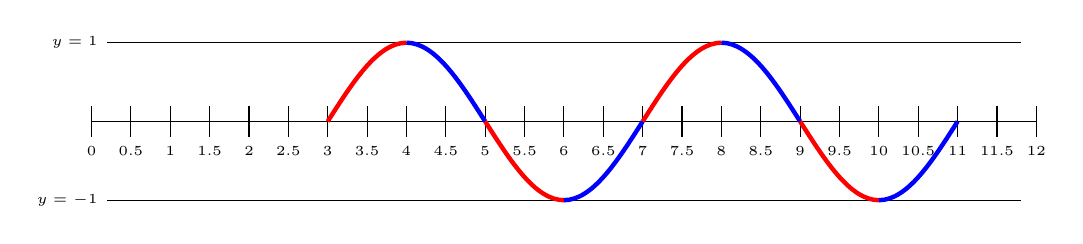
\begin{tikzpicture}
    \draw (0,0) -- (12,0);
    \draw (0.2,1)node[left,font=\tiny] {$y=1$} -- (11.8,1);
    \draw (0.2,-1)node[left,font=\tiny] {$y=-1$} -- (11.8,-1); 
    \foreach \x in {0,0.5,...,12}{
    \draw (\x,-0.2)node [below,font=\tiny,] {\x} -- (\x,0.2) ;
    }
    \draw[ultra thick, red] (3,0) sin (4,1);    %% the real business in this line
    \draw[ultra thick, blue] (4,1) cos (5,0);    %% the real business in this line
    \draw[ultra thick, red] (5,0) sin (6,-1);    %% the real business in this line
    \draw[ultra thick, blue] (6,-1) cos (7,0);    %% the real business in this line
    \draw[ultra thick, red] (7,0)  sin (8,1);    %% the real business in this line
    \draw[ultra thick, blue] (8,1) cos (9,0);    %% the real business in this line
    \draw[ultra thick, red] (9,0) sin (10,-1);    %% the real business in this line
    \draw[ultra thick, blue] (10,-1) cos (11,0);    %% the real business in this line
    \end{tikzpicture}
\end{figure}




\section{Summary}
\label{sec:ch_3_summary}

This is a topic sentence followed by explanation, elaboration and examples to summarise the second subsection. The last sentence of this paragraph shall introduce the next paragraph. \lipsum[1]

This is a topic sentence followed by explanation, elaboration and examples to summarise the third subsection. The last sentence of this paragraph shall introduce the next paragraph. \lipsum[1]

This is a topic sentence followed by explanation, elaboration and examples to summarise the fourth subsection. The last sentence of this paragraph shall introduce the next chapter. \lipsum[1]





%*****************************************
%*****************************************
%*****************************************
%*****************************************
%*****************************************






\cleardoublepage



%*******************************************************
% This program is free software: you can redistribute it and/or modify
% it under the terms of the GNU General Public License as published by
% the Free Software Foundation, either version 3 of the License, or
% (at your option) any later version.
%
% This program is distributed in the hope that it will be useful,
% but WITHOUT ANY WARRANTY; without even the implied warranty of
% MERCHANTABILITY or FITNESS FOR A PARTICULAR PURPOSE.  See the
% GNU General Public License for more details.
%
% You should have received a copy of the GNU General Public License
% along with this program.  If not, see <http://www.gnu.org/licenses/>.
%************************************************
\chapter{This is chapter four}
\label{ch:name4}
%************************************************

\begin{flushright}
{\slshape Lorem ipsum dolor sit amet, consectetuer adipiscing.}\\
{\slshape Aenean commodo ligula eget dolor. Aenean massa.}\\
% This generate dummy text. Remove this line and replace by your quote.
\medskip
--- John Doe,\\
Unified Theory of the Important Theories,\\
{\slshape An Important Journal},\\
Vol.~123, pp.~1234--1243, Dec.~2016.\\
\end{flushright}

\bigskip


%\minitoc\nomtcpagenumbers

%\marginpar{\myTitle \myVersion}

\section{Introduction}
\label{sec:ch_4_introduction}

\citet{Berg2016} argues that this is a topic sentence followed by explanation, elaboration and examples to introduce the next three subsections. The last sentence of this paragraph shall introduce the next paragraph. \lipsum[1]

This is a topic sentence followed by explanation, elaboration and examples to introduce the next three subsections \citep{Collins2016}. The last sentence of this paragraph shall introduce the next paragraph. \lipsum[1]

\citet{Graham2016} and \citet{Grant2016} assert that this is a topic sentence followed by explanation, elaboration and examples to introduce the next three subsections. The last sentence of this paragraph shall introduce the next paragraph. \lipsum[1]

\section{First main stuff}
\label{sec:ch_4_firstmain}

This is a topic sentence followed by explanation, elaboration and examples to introduce this paragraph \citep{Haney2016}. The last sentence of this paragraph shall introduce the next paragraph. \lipsum[1]

This is a topic sentence followed by explanation, elaboration and examples to introduce this paragraph \citep{Jordan2016,Morgan2016}. The last sentence of this paragraph shall introduce the next paragraph. \lipsum[1]

This is a topic sentence followed by explanation, elaboration and examples to introduce this paragraph. The last sentence of this paragraph shall introduce the next paragraph. \lipsum[1]

\section{Second main stuff}
\label{sec:ch_4_secondmain}

This is a topic sentence followed by explanation, elaboration and examples to introduce this paragraph \citep{Scott2016}. The last sentence of this paragraph shall introduce the next paragraph. \lipsum[1]

\begin{figure}[h]
    \centering
    \includegraphics[width=0.9\textwidth]{imageFiles/imageExample}
    \caption{A copy from previous image}
    \label{fig:copycurve}
\end{figure}
 
As \citet{Wells2016} and \citet{Williamson2016} denotated in the figure \ref{fig:copycurve}, the 
function grows near 0. Also, in the page \pageref{fig:curve} 
is the same example in figure \ref{fig:curve}.

This is a topic sentence followed by explanation, elaboration and examples to introduce this paragraph \citep{Stewart2016}. The last sentence of this paragraph shall introduce the next paragraph. \lipsum[1]

This is a topic sentence followed by explanation, elaboration and examples to introduce this paragraph \citep{Gallagher2016}. The last sentence of this paragraph shall introduce the next paragraph. \lipsum[1]

\section{Third main stuff}
\label{sec:ch_4_thirdmain}


This is a topic sentence followed by explanation, elaboration and examples to introduce this paragraph. The last sentence of this paragraph shall introduce the next paragraph. \lipsum[1]

This is a topic sentence followed by explanation, elaboration and examples to introduce this paragraph. The last sentence of this paragraph shall introduce the next paragraph. \lipsum[1]

This is a topic sentence followed by explanation, elaboration and examples to introduce this paragraph. The last sentence of this paragraph shall introduce the next paragraph. \lipsum[1]

\section{Summary}
\label{sec:ch_4_summary}


This is a topic sentence followed by explanation, elaboration and examples to summarise the second subsection. The last sentence of this paragraph shall introduce the next paragraph. \lipsum[1]

This is a topic sentence followed by explanation, elaboration and examples to summarise the third subsection. The last sentence of this paragraph shall introduce the next paragraph. \lipsum[1]

This is a topic sentence followed by explanation, elaboration and examples to summarise the fourth subsection. The last sentence of this paragraph shall introduce the next chapter. \lipsum[1]



%*****************************************
%*****************************************
%*****************************************
%*****************************************
%*****************************************






\cleardoublepage

\include{chapters/chapter5}

\cleardoublepage

\include{chapters/chapter6}

%*******************************************************
% Appendix
%*******************************************************

\appendix
%************************************************
\chapter{List of MC samples}
\label{ch:appendixOne}
%************************************************

\section{List of data samples}
\label{sec:List_Data}
The following Good Run Lists (GRL) are used.
\begin{itemize}
\item {\ttfamily\scriptsize data15\_13TeV.periodAllYear\_DetStatus-v79-repro20-02\_DQDefects-00-02-02\_PHYS\_StandardGRL\_All\_Good\_25ns.xml} for 2015 data.
\item {\ttfamily\scriptsize data16\_13TeV.periodAllYear\_DetStatus-v89-pro21-01\_DQDefects-00-02-04\_PHYS\_StandardGRL\_All\_Good\_25ns.xml} for 2016 data.
\end{itemize}
The following are the list of data samples used.
\scriptsize
\begin{verbatim}
data15_13TeV.periodD.physics_Main.PhysCont.DAOD_SUSY2.grp15_v02_p2950
data15_13TeV.periodE.physics_Main.PhysCont.DAOD_SUSY2.grp15_v02_p2950
data15_13TeV.periodF.physics_Main.PhysCont.DAOD_SUSY2.grp15_v02_p2950
data15_13TeV.periodG.physics_Main.PhysCont.DAOD_SUSY2.grp15_v02_p2950
data15_13TeV.periodH.physics_Main.PhysCont.DAOD_SUSY2.grp15_v02_p2950
data15_13TeV.periodJ.physics_Main.PhysCont.DAOD_SUSY2.grp15_v02_p2950
data16_13TeV.periodA.physics_Main.PhysCont.DAOD_SUSY2.grp16_v02_p2950
data16_13TeV.periodB.physics_Main.PhysCont.DAOD_SUSY2.grp16_v02_p2950
data16_13TeV.periodC.physics_Main.PhysCont.DAOD_SUSY2.grp16_v02_p2950
data16_13TeV.periodD.physics_Main.PhysCont.DAOD_SUSY2.grp16_v02_p2950
data16_13TeV.periodE.physics_Main.PhysCont.DAOD_SUSY2.grp16_v02_p2950
data16_13TeV.periodF.physics_Main.PhysCont.DAOD_SUSY2.grp16_v02_p2950
data16_13TeV.periodG.physics_Main.PhysCont.DAOD_SUSY2.grp16_v02_p2950
data16_13TeV.periodI.physics_Main.PhysCont.DAOD_SUSY2.grp16_v02_p2950
data16_13TeV.periodK.physics_Main.PhysCont.DAOD_SUSY2.grp16_v02_p2950
data16_13TeV.periodL.physics_Main.PhysCont.DAOD_SUSY2.grp16_v02_p2950
\end{verbatim}
\normalsize

\section{List of background MC samples}
\label{sec:MCBG}
\begin{table}[htbp]
\begin{center}
\tiny
\scalebox{0.7}{
\begin{tabular}{ccccccc}
\hline
Dataset ID & Process & Tags & Cross section [pb] & $k$-factor & Generator efficiency & $ \mathcal{L}_{int} [\mathrm{fb}^{-1}]$ \\
\hline
364156 & Sherpa\_221\_NNPDF30NNLO\_Wmunu\_MAXHTPTV0\_70\_CVetoBVeto & e5340\_s2726\_r7772\_r7676\_p2949 & 19143.0000 & 0.97 & 0.824 & 1.616 \\ 
364157 & Sherpa\_221\_NNPDF30NNLO\_Wmunu\_MAXHTPTV0\_70\_CFilterBVeto & e5340\_s2726\_r7772\_r7676\_p2949 & 19121.0000 & 0.97 & 0.130 & 4.071 \\ 
364158 & Sherpa\_221\_NNPDF30NNLO\_Wmunu\_MAXHTPTV0\_70\_BFilter & e5340\_s2726\_r7772\_r7676\_p2949 & 19135.0000 & 0.97 & 0.044 & 21.032 \\ 
364159 & Sherpa\_221\_NNPDF30NNLO\_Wmunu\_MAXHTPTV70\_140\_CVetoBVeto & e5340\_s2726\_r7772\_r7676\_p2949 & 944.8500 & 0.97 & 0.675 & 23.912 \\ 
364160 & Sherpa\_221\_NNPDF30NNLO\_Wmunu\_MAXHTPTV70\_140\_CFilterBVeto & e5340\_s2726\_r7772\_r7676\_p2949 & 937.7800 & 0.97 & 0.235 & 46.173 \\ 
364161 & Sherpa\_221\_NNPDF30NNLO\_Wmunu\_MAXHTPTV70\_140\_BFilter & e5340\_s2726\_r7772\_r7676\_p2949 & 944.6300 & 0.97 & 0.076 & 283.269 \\ 
364162 & Sherpa\_221\_NNPDF30NNLO\_Wmunu\_MAXHTPTV140\_280\_CVetoBVeto & e5340\_s2726\_r7772\_r7676\_p2949 & 339.5400 & 0.97 & 0.626 & 47.919 \\ 
364163 & Sherpa\_221\_NNPDF30NNLO\_Wmunu\_MAXHTPTV140\_280\_CFilterBVeto & e5340\_s2726\_r7772\_r7676\_p2949 & 340.0600 & 0.97 & 0.289 & 77.568 \\ 
364164 & Sherpa\_221\_NNPDF30NNLO\_Wmunu\_MAXHTPTV140\_280\_BFilter & e5340\_s2726\_r7772\_r7676\_p2949 & 339.5400 & 0.97 & 0.109 & 686.449 \\ 
364165 & Sherpa\_221\_NNPDF30NNLO\_Wmunu\_MAXHTPTV280\_500\_CVetoBVeto & e5340\_s2726\_r7772\_r7676\_p2949 & 72.0670 & 0.97 & 0.546 & 129.289 \\ 
364166 & Sherpa\_221\_NNPDF30NNLO\_Wmunu\_MAXHTPTV280\_500\_CFilterBVeto & e5340\_s2726\_r7772\_r7676\_p2949 & 72.1980 & 0.97 & 0.317 & 133.034 \\ 
364167 & Sherpa\_221\_NNPDF30NNLO\_Wmunu\_MAXHTPTV280\_500\_BFilter & e5340\_s2726\_r7772\_r7676\_p2949 & 72.0450 & 0.97 & 0.133 & 317.464 \\ 
364168 & Sherpa\_221\_NNPDF30NNLO\_Wmunu\_MAXHTPTV500\_1000 & e5340\_s2726\_r7772\_r7676\_p2949 & 15.0100 & 0.97 & 1.000 & 405.866 \\ 
364169 & Sherpa\_221\_NNPDF30NNLO\_Wmunu\_MAXHTPTV1000\_E\_CMS & e5340\_s2726\_r7772\_r7676\_p2949 & 1.2344 & 0.97 & 1.000 & 3305.737 \\ 
364170 & Sherpa\_221\_NNPDF30NNLO\_Wenu\_MAXHTPTV0\_70\_CVetoBVeto & e5340\_s2726\_r7772\_r7676\_p2949 & 19127.0000 & 0.97 & 0.824 & 1.617 \\ 
364171 & Sherpa\_221\_NNPDF30NNLO\_Wenu\_MAXHTPTV0\_70\_CFilterBVeto & e5340\_s2726\_r7772\_r7676\_p2949 & 19130.0000 & 0.97 & 0.130 & 4.074 \\ 
364172 & Sherpa\_221\_NNPDF30NNLO\_Wenu\_MAXHTPTV0\_70\_BFilter & e5340\_s2726\_r7772\_r7676\_p2949 & 19135.0000 & 0.97 & 0.044 & 20.272 \\ 
364173 & Sherpa\_221\_NNPDF30NNLO\_Wenu\_MAXHTPTV70\_140\_CVetoBVeto & e5340\_s2726\_r7772\_r7676\_p2949 & 942.5800 & 0.97 & 0.669 & 23.973 \\ 
364174 & Sherpa\_221\_NNPDF30NNLO\_Wenu\_MAXHTPTV70\_140\_CFilterBVeto & e5340\_s2726\_r7772\_r7676\_p2949 & 945.6700 & 0.97 & 0.228 & 46.963 \\ 
364175 & Sherpa\_221\_NNPDF30NNLO\_Wenu\_MAXHTPTV70\_140\_BFilter & e5340\_s2726\_r7772\_r7676\_p2949 & 945.1500 & 0.97 & 0.103 & 103.368 \\ 
364176 & Sherpa\_221\_NNPDF30NNLO\_Wenu\_MAXHTPTV140\_280\_CVetoBVeto & e5340\_s2726\_r7772\_r7676\_p2949 & 339.8100 & 0.97 & 0.597 & 50.200 \\ 
364177 & Sherpa\_221\_NNPDF30NNLO\_Wenu\_MAXHTPTV140\_280\_CFilterBVeto & e5340\_s2726\_r7772\_r7676\_p2949 & 339.8700 & 0.97 & 0.290 & 77.584 \\ 
364178 & Sherpa\_221\_NNPDF30NNLO\_Wenu\_MAXHTPTV140\_280\_BFilter & e5340\_s2726\_r7772\_r7676\_p2949 & 339.4800 & 0.97 & 0.109 & 687.518 \\ 
364179 & Sherpa\_221\_NNPDF30NNLO\_Wenu\_MAXHTPTV280\_500\_CVetoBVeto & e5340\_s2726\_r7772\_r7676\_p2949 & 72.0840 & 0.97 & 0.544 & 129.323 \\ 
364180 & Sherpa\_221\_NNPDF30NNLO\_Wenu\_MAXHTPTV280\_500\_CFilterBVeto & e5340\_s2726\_r7772\_r7676\_p2949 & 72.1280 & 0.97 & 0.317 & 133.693 \\ 
364181 & Sherpa\_221\_NNPDF30NNLO\_Wenu\_MAXHTPTV280\_500\_BFilter & e5340\_s2726\_r7772\_r7676\_p2949 & 72.1130 & 0.97 & 0.134 & 315.726 \\ 
364182 & Sherpa\_221\_NNPDF30NNLO\_Wenu\_MAXHTPTV500\_1000 & e5340\_s2726\_r7772\_r7676\_p2949 & 15.2240 & 0.97 & 1.000 & 400.587 \\ 
364183 & Sherpa\_221\_NNPDF30NNLO\_Wenu\_MAXHTPTV1000\_E\_CMS & e5340\_s2726\_r7772\_r7676\_p2949 & 1.2334 & 0.97 & 1.000 & 3298.389 \\ 
364184 & Sherpa\_221\_NNPDF30NNLO\_Wtaunu\_MAXHTPTV0\_70\_CVetoBVeto & e5340\_s2726\_r7772\_r7676\_p2949 & 19152.0000 & 0.97 & 0.825 & 1.617 \\ 
364185 & Sherpa\_221\_NNPDF30NNLO\_Wtaunu\_MAXHTPTV0\_70\_CFilterBVeto & e5340\_s2726\_r7772\_r7676\_p2949 & 19153.0000 & 0.97 & 0.129 & 4.105 \\ 
364186 & Sherpa\_221\_NNPDF30NNLO\_Wtaunu\_MAXHTPTV0\_70\_BFilter & e5340\_s2726\_r7772\_r7676\_p2949 & 19163.0000 & 0.97 & 0.045 & 20.834 \\ 
364187 & Sherpa\_221\_NNPDF30NNLO\_Wtaunu\_MAXHTPTV70\_140\_CVetoBVeto & e5340\_s2726\_r7772\_r7676\_p2949 & 947.6500 & 0.97 & 0.674 & 23.903 \\ 
364188 & Sherpa\_221\_NNPDF30NNLO\_Wtaunu\_MAXHTPTV70\_140\_CFilterBVeto & e5340\_s2726\_r7772\_r7676\_p2949 & 946.7300 & 0.97 & 0.222 & 48.307 \\ 
364189 & Sherpa\_221\_NNPDF30NNLO\_Wtaunu\_MAXHTPTV70\_140\_BFilter & e5340\_s2726\_r7772\_r7676\_p2949 & 943.3000 & 0.97 & 0.104 & 103.602 \\ 
364190 & Sherpa\_221\_NNPDF30NNLO\_Wtaunu\_MAXHTPTV140\_280\_CVetoBVeto & e5340\_s2726\_r7772\_r7676\_p2949 & 339.3600 & 0.97 & 0.596 & 50.427 \\ 
364191 & Sherpa\_221\_NNPDF30NNLO\_Wtaunu\_MAXHTPTV140\_280\_CFilterBVeto & e5340\_s2726\_r7772\_r7676\_p2949 & 339.6300 & 0.97 & 0.290 & 76.903 \\ 
364192 & Sherpa\_221\_NNPDF30NNLO\_Wtaunu\_MAXHTPTV140\_280\_BFilter & e5340\_s2726\_r7772\_r7676\_p2949 & 339.5400 & 0.97 & 0.118 & 632.798 \\ 
364193 & Sherpa\_221\_NNPDF30NNLO\_Wtaunu\_MAXHTPTV280\_500\_CVetoBVeto & e5340\_s2726\_r7772\_r7676\_p2949 & 72.0650 & 0.92 & 0.546 & 136.270 \\ 
364194 & Sherpa\_221\_NNPDF30NNLO\_Wtaunu\_MAXHTPTV280\_500\_CFilterBVeto & e5340\_s2726\_r7772\_r7676\_p2949 & 71.9760 & 0.97 & 0.316 & 133.773 \\ 
364195 & Sherpa\_221\_NNPDF30NNLO\_Wtaunu\_MAXHTPTV280\_500\_BFilter & e5340\_s2726\_r7772\_r7676\_p2949 & 72.0260 & 0.97 & 0.134 & 314.868 \\ 
364196 & Sherpa\_221\_NNPDF30NNLO\_Wtaunu\_MAXHTPTV500\_1000 & e5340\_s2726\_r7772\_r7676\_p2949 & 15.0460 & 0.97 & 1.000 & 407.258 \\ 
364197 & Sherpa\_221\_NNPDF30NNLO\_Wtaunu\_MAXHTPTV1000\_E\_CMS & e5340\_s2726\_r7772\_r7676\_p2949 & 1.2339 & 0.97 & 1.000 & 3296.218 \\ 
\hline
\end{tabular}}
\end{center}
\caption{List of simulated W+jets processes}
\label{table:wjets}
\end{table}

\begin{table}[htbp]
\begin{center}
\tiny
\scalebox{0.7}{
\begin{tabular}{ccccccc}
\hline
Dataset ID & Process & Tags & Cross section [pb] & $k$-factor & Generator efficiency & $ \mathcal{L}_{int} [\mathrm{fb}^{-1}]$ \\
\hline
364100 & Sherpa\_221\_NNPDF30NNLO\_Zmumu\_MAXHTPTV0\_70\_CVetoBVeto & e5271\_s2726\_r7772\_r7676\_p2949 & 1983.0000 & 0.98 & 0.822 & 4.964 \\ 
364101 & Sherpa\_221\_NNPDF30NNLO\_Zmumu\_MAXHTPTV0\_70\_CFilterBVeto & e5271\_s2726\_r7772\_r7676\_p2949 & 1978.4000 & 0.98 & 0.113 & 22.540 \\ 
364102 & Sherpa\_221\_NNPDF30NNLO\_Zmumu\_MAXHTPTV0\_70\_BFilter & e5271\_s2726\_r7772\_r7676\_p2949 & 1982.2000 & 0.98 & 0.064 & 63.719 \\ 
364103 & Sherpa\_221\_NNPDF30NNLO\_Zmumu\_MAXHTPTV70\_140\_CVetoBVeto & e5271\_s2726\_r7772\_r7676\_p2949 & 108.9200 & 0.98 & 0.689 & 80.890 \\ 
364104 & Sherpa\_221\_NNPDF30NNLO\_Zmumu\_MAXHTPTV70\_140\_CFilterBVeto & e5271\_s2726\_r7772\_r7676\_p2949 & 109.4200 & 0.98 & 0.186 & 99.279 \\ 
364105 & Sherpa\_221\_NNPDF30NNLO\_Zmumu\_MAXHTPTV70\_140\_BFilter & e5271\_s2726\_r7772\_r7676\_p2949 & 108.9100 & 0.98 & 0.114 & 488.459 \\ 
364106 & Sherpa\_221\_NNPDF30NNLO\_Zmumu\_MAXHTPTV140\_280\_CVetoBVeto & e5271\_s2726\_r7772\_r7676\_p2949 & 39.8780 & 0.98 & 0.609 & 208.736 \\ 
364107 & Sherpa\_221\_NNPDF30NNLO\_Zmumu\_MAXHTPTV140\_280\_CFilterBVeto & e5271\_s2726\_r7772\_r7676\_p2949 & 39.7950 & 0.98 & 0.233 & 326.653 \\ 
364108 & Sherpa\_221\_NNPDF30NNLO\_Zmumu\_MAXHTPTV140\_280\_BFilter & e5271\_s2726\_r7772\_r7676\_p2949 & 39.9080 & 0.98 & 0.146 & 2169.169 \\ 
364109 & Sherpa\_221\_NNPDF30NNLO\_Zmumu\_MAXHTPTV280\_500\_CVetoBVeto & e5271\_s2726\_r7772\_r7676\_p2949 & 8.5375 & 0.98 & 0.559 & 423.925 \\ 
364110 & Sherpa\_221\_NNPDF30NNLO\_Zmumu\_MAXHTPTV280\_500\_CFilterBVeto & e5271\_s2726\_r7772\_r7676\_p2949 & 8.5403 & 0.98 & 0.265 & 446.324 \\ 
364111 & Sherpa\_221\_NNPDF30NNLO\_Zmumu\_MAXHTPTV280\_500\_BFilter & e5271\_s2726\_r7772\_r7676\_p2949 & 8.4932 & 0.98 & 0.176 & 1355.672 \\ 
364112 & Sherpa\_221\_NNPDF30NNLO\_Zmumu\_MAXHTPTV500\_1000 & e5271\_s2726\_r7772\_r7676\_p2949 & 1.7881 & 0.98 & 1.000 & 1697.947 \\ 
364113 & Sherpa\_221\_NNPDF30NNLO\_Zmumu\_MAXHTPTV1000\_E\_CMS & e5271\_s2726\_r7772\_r7676\_p2949 & 0.1477 & 0.98 & 1.000 & 6860.515 \\ 
364114 & Sherpa\_221\_NNPDF30NNLO\_Zee\_MAXHTPTV0\_70\_CVetoBVeto & e5299\_s2726\_r7772\_r7676\_p2949 & 1981.8000 & 0.98 & 0.821 & 4.979 \\ 
364115 & Sherpa\_221\_NNPDF30NNLO\_Zee\_MAXHTPTV0\_70\_CFilterBVeto & e5299\_s2726\_r7772\_r7676\_p2949 & 1980.8000 & 0.98 & 0.113 & 22.646 \\ 
364116 & Sherpa\_221\_NNPDF30NNLO\_Zee\_MAXHTPTV0\_70\_BFilter & e5299\_s2726\_r7772\_r7676\_p2949 & 1981.7000 & 0.98 & 0.064 & 63.937 \\ 
364117 & Sherpa\_221\_NNPDF30NNLO\_Zee\_MAXHTPTV70\_140\_CVetoBVeto & e5299\_s2726\_r7772\_r7676\_p2949 & 110.5000 & 0.98 & 0.690 & 79.645 \\ 
364118 & Sherpa\_221\_NNPDF30NNLO\_Zee\_MAXHTPTV70\_140\_CFilterBVeto & e5299\_s2726\_r7772\_r7676\_p2949 & 110.6300 & 0.98 & 0.184 & 99.477 \\ 
364119 & Sherpa\_221\_NNPDF30NNLO\_Zee\_MAXHTPTV70\_140\_BFilter & e5299\_s2726\_r7772\_r7676\_p2949 & 110.3100 & 0.98 & 0.114 & 475.689 \\ 
364120 & Sherpa\_221\_NNPDF30NNLO\_Zee\_MAXHTPTV140\_280\_CVetoBVeto & e5299\_s2726\_r7772\_r7676\_p2949 & 40.7310 & 0.98 & 0.615 & 202.772 \\ 
364121 & Sherpa\_221\_NNPDF30NNLO\_Zee\_MAXHTPTV140\_280\_CFilterBVeto & e5299\_s2726\_r7772\_r7676\_p2949 & 40.6700 & 0.98 & 0.230 & 324.184 \\ 
364122 & Sherpa\_221\_NNPDF30NNLO\_Zee\_MAXHTPTV140\_280\_BFilter & e5299\_s2726\_r7772\_r7676\_p2949 & 40.6430 & 0.98 & 0.150 & 2078.998 \\ 
364123 & Sherpa\_221\_NNPDF30NNLO\_Zee\_MAXHTPTV280\_500\_CVetoBVeto & e5299\_s2726\_r7772\_r7676\_p2949 & 8.6743 & 0.98 & 0.561 & 407.078 \\ 
364124 & Sherpa\_221\_NNPDF30NNLO\_Zee\_MAXHTPTV280\_500\_CFilterBVeto & e5299\_s2726\_r7772\_r7676\_p2949 & 8.6711 & 0.98 & 0.263 & 444.808 \\ 
364125 & Sherpa\_221\_NNPDF30NNLO\_Zee\_MAXHTPTV280\_500\_BFilter & e5299\_s2726\_r7772\_r7676\_p2949 & 8.6766 & 0.98 & 0.172 & 1356.645 \\ 
364126 & Sherpa\_221\_NNPDF30NNLO\_Zee\_MAXHTPTV500\_1000 & e5299\_s2726\_r7772\_r7676\_p2949 & 1.8081 & 0.98 & 1.000 & 1686.255 \\ 
364127 & Sherpa\_221\_NNPDF30NNLO\_Zee\_MAXHTPTV1000\_E\_CMS & e5299\_s2726\_r7772\_r7676\_p2949 & 0.1486 & 0.98 & 1.000 & 6819.879 \\ 
364128 & Sherpa\_221\_NNPDF30NNLO\_Ztautau\_MAXHTPTV0\_70\_CVetoBVeto & e5307\_s2726\_r7772\_r7676\_p2949 & 1981.6000 & 0.98 & 0.821 & 4.982 \\ 
364129 & Sherpa\_221\_NNPDF30NNLO\_Ztautau\_MAXHTPTV0\_70\_CFilterBVeto & e5307\_s2726\_r7772\_r7676\_p2949 & 1978.8000 & 0.98 & 0.113 & 22.633 \\ 
364130 & Sherpa\_221\_NNPDF30NNLO\_Ztautau\_MAXHTPTV0\_70\_BFilter & e5307\_s2726\_r7772\_r7676\_p2949 & 1981.8000 & 0.98 & 0.064 & 63.352 \\ 
364131 & Sherpa\_221\_NNPDF30NNLO\_Ztautau\_MAXHTPTV70\_140\_CVetoBVeto & e5307\_s2726\_r7772\_r7676\_p2949 & 110.3700 & 0.98 & 0.689 & 80.065 \\ 
364132 & Sherpa\_221\_NNPDF30NNLO\_Ztautau\_MAXHTPTV70\_140\_CFilterBVeto & e5307\_s2726\_r7772\_r7676\_p2949 & 110.5100 & 0.98 & 0.183 & 99.508 \\ 
364133 & Sherpa\_221\_NNPDF30NNLO\_Ztautau\_MAXHTPTV70\_140\_BFilter & e5307\_s2726\_r7772\_r7676\_p2949 & 110.8700 & 0.98 & 0.111 & 493.213 \\ 
364134 & Sherpa\_221\_NNPDF30NNLO\_Ztautau\_MAXHTPTV140\_280\_CVetoBVeto & e5307\_s2726\_r7772\_r7676\_p2949 & 40.7810 & 0.98 & 0.608 & 204.914 \\ 
364135 & Sherpa\_221\_NNPDF30NNLO\_Ztautau\_MAXHTPTV140\_280\_CFilterBVeto & e5307\_s2726\_r7772\_r7676\_p2949 & 40.7400 & 0.98 & 0.229 & 326.848 \\ 
364136 & Sherpa\_221\_NNPDF30NNLO\_Ztautau\_MAXHTPTV140\_280\_BFilter & e5307\_s2726\_r7772\_r7676\_p2949 & 40.7610 & 0.98 & 0.134 & 923.313 \\ 
364137 & Sherpa\_221\_NNPDF30NNLO\_Ztautau\_MAXHTPTV280\_500\_CVetoBVeto & e5307\_s2726\_r7772\_r7676\_p2949 & 8.5502 & 0.98 & 0.560 & 422.313 \\ 
364138 & Sherpa\_221\_NNPDF30NNLO\_Ztautau\_MAXHTPTV280\_500\_CFilterBVeto & e5313\_s2726\_r7772\_r7676\_p2949 & 8.6707 & 0.98 & 0.262 & 444.352 \\ 
364139 & Sherpa\_221\_NNPDF30NNLO\_Ztautau\_MAXHTPTV280\_500\_BFilter & e5313\_s2726\_r7772\_r7676\_p2949 & 8.6804 & 0.98 & 0.173 & 1347.705 \\ 
364140 & Sherpa\_221\_NNPDF30NNLO\_Ztautau\_MAXHTPTV500\_1000 & e5307\_s2726\_r7772\_r7676\_p2949 & 1.8096 & 0.98 & 1.000 & 1668.876 \\ 
364141 & Sherpa\_221\_NNPDF30NNLO\_Ztautau\_MAXHTPTV1000\_E\_CMS & e5307\_s2726\_r7772\_r7676\_p2949 & 0.1483 & 0.98 & 1.000 & 6775.146 \\ 
\hline
\end{tabular}}
\end{center}
\caption{List of simulated Z+jets processes}
\label{table:zjets}
\end{table} 

\begin{table}[htbp]
\begin{center}
\tiny
\scalebox{0.7}{
\begin{tabular}{ccccccc} 
\hline
Dataset ID & Process & Tags & Cross section [pb] & $k$-factor & Generator efficiency & $ \mathcal{L}_{int} [\mathrm{fb}^{-1}]$ \\
\hline
410011 & PowhegPythiaEvtGen\_P2012\_singletop\_tchan\_lept\_top & e3824\_s2608\_s2183\_r7725\_r7676\_p2949 & 43.7390 & 1.01 & 1.000 & 112.937 \\ 
410012 & PowhegPythiaEvtGen\_P2012\_singletop\_tchan\_lept\_antitop & e3824\_s2608\_s2183\_r7725\_r7676\_p2949 & 25.7780 & 1.02 & 1.000 & 189.903 \\ 
410015 & PowhegPythiaEvtGen\_P2012\_Wt\_dilepton\_top & e3753\_s2608\_s2183\_r7725\_r7676\_p2949 & 3.5835 & 1.05 & 1.000 & 262.959 \\ 
410016 & PowhegPythiaEvtGen\_P2012\_Wt\_dilepton\_antitop & e3753\_s2608\_s2183\_r7725\_r7676\_p2949 & 3.5814 & 1.05 & 1.000 & 262.690 \\ 
410026 & PowhegPythiaEvtGen\_P2012\_SingleTopSchan\_noAllHad\_antitop & e3998\_s2608\_s2183\_r7725\_r7676\_p2949 & 1.2615 & 1.02 & 1.000 & 772.453 \\ 
410025 & PowhegPythiaEvtGen\_P2012\_SingleTopSchan\_noAllHad\_top & e3998\_s2608\_s2183\_r7725\_r7676\_p2949 & 2.0517 & 1.00 & 1.000 & 484.101 \\ 
\hline
\end{tabular}}
\end{center}
\caption{List of simulated single-top processes}
\label{table:singletop}
\end{table} 

\begin{table}[htbp]
\begin{center}
\tiny
\scalebox{0.7}{
\begin{tabular}{ccccccc} 
\hline
Dataset ID & Process & Tags & Cross section [pb] & $k$-factor & Generator efficiency & $ \mathcal{L}_{int} [\mathrm{fb}^{-1}]$ \\
\hline
410000 & PowhegPythiaEvtGen\_P2012\_ttbar\_hdamp172p5\_nonallhad & e3698\_s2608\_s2183\_r7725\_r7676\_p2949 & 696.1100 & 1.19 & 0.543 & 109.345 \\ 
\hline
\end{tabular}}
\end{center}
\caption{List of the simulated $t\bar{t}$ sample}
\label{table:ttbar}
\end{table} 

\begin{table}[htbp]
\begin{center}
\tiny
\scalebox{0.7}{
\begin{tabular}{ccccccc} 
\hline
Dataset ID & Process & Tags & Cross section [pb] & $k$-factor & Generator efficiency & $ \mathcal{L}_{int} [\mathrm{fb}^{-1}]$ \\
\hline
410218 & aMcAtNloPythia8EvtGen\_MEN30NLO\_A14N23LO\_ttee & e5070\_s2726\_r7772\_r7676\_p2949 & 0.0369 & 1.12 & 1.000 & 34099.359 \\ 
410219 & aMcAtNloPythia8EvtGen\_MEN30NLO\_A14N23LO\_ttmumu & e5070\_s2726\_r7772\_r7676\_p2949 & 0.0369 & 1.12 & 1.000 & 34112.250 \\ 
410220 & aMcAtNloPythia8EvtGen\_MEN30NLO\_A14N23LO\_tttautau & e5070\_s2726\_r7772\_r7676\_p2949 & 0.0366 & 1.12 & 1.000 & 22792.877 \\ 
410155 & aMcAtNloPythia8EvtGen\_MEN30NLO\_A14N23LO\_ttW & e5070\_s2726\_r7772\_r7676\_p2949 & 0.5483 & 1.10 & 1.000 & 12423.357 \\ 
410081 & MadGraphPythia8EvtGen\_A14NNPDF23\_ttbarWW & e4111\_s2608\_s2183\_r7725\_r7676\_p2949 & 0.0081 & 1.22 & 1.000 & 5048.439 \\ 
407321 & MadGraphPythia8EvtGen\_A14NNPDF23LO\_ttbarWll & e5536\_s2726\_r7772\_r7676\_p2949 & 0.0003 & 1.34 & 1.000 & 84165.641 \\ 
\hline
\end{tabular}}
\end{center}
\caption{List of simulated $t\bar{t}$ plus vector boson processes}
\label{table:ttv}
\end{table} 

\begin{table}[htbp]
\begin{center}
\tiny
\scalebox{0.7}{
\begin{tabular}{clccccc} 
\hline
Dataset ID & Process & Tags & Cross section [pb] & $k$-factor & Generator efficiency & $ \mathcal{L}_{int} [\mathrm{fb}^{-1}]$ \\
\hline
341079 & PowhegPythia8EvtGen\_CT10\_AZNLOCTEQ6L1\_ggH125\_WWlvlv\_EF\_15\_5 & e3871\_s2608\_s2183\_r7772\_r7676\_p2949 & 0.9902 & 1.00 & 0.491 & 983.382 \\ 
341122 & PowhegPythia8EvtGen\_CT10\_AZNLOCTEQ6L1\_ggH125\_tautaull & e3935\_s2608\_s2183\_r7772\_r7676\_p2949 & 1.9081 & 1.45 & 0.123 & 4467.140 \\ 
341195 & PowhegPythia8EvtGen\_CT10\_AZNLOCTEQ6L1\_ggH125\_mumu & e3945\_s2608\_s2183\_r7772\_r7676\_p2949 & 0.0066 & 1.45 & 1.000 & 99495.922 \\ 
342178 & PowhegPythia8EvtGen\_CT10\_AZNLOCTEQ6L1\_ggH125\_ee & e4158\_s2608\_r7772\_r7676\_p2949 & 0.0000 & 1.45 & 1.000 & 293359648.000 \\ 
341080 & PowhegPythia8EvtGen\_CT10\_AZNLOCTEQ6L1\_VBFH125\_WWlvlv\_EF\_15\_5 & e3871\_s2608\_s2183\_r7772\_r7676\_p2949 & 0.0848 & 1.00 & 0.510 & 5774.853 \\ 
341155 & PowhegPythia8EvtGen\_CT10\_AZNLOCTEQ6L1\_VBFH125\_tautaull & e3888\_s2608\_s2183\_r7772\_r7676\_p2949 & 0.2420 & 0.98 & 0.123 & 71518.055 \\ 
341206 & PowhegPythia8EvtGen\_CT10\_AZNLOCTEQ6L1\_VBFH125\_mumu & e3945\_s2608\_s2183\_r7772\_r7676\_p2949 & 0.0009 & 0.96 & 1.000 & 998280.062 \\ 
342189 & PowhegPythia8EvtGen\_CT10\_AZNLOCTEQ6L1\_VBFH125\_ee & e4158\_s2608\_r7772\_r7676\_p2949 & 0.0000 & 0.98 & 1.000 & 5208568320.000 \\ 
342284 & Pythia8EvtGen\_A14NNPDF23LO\_WH125\_inc & e4246\_s2608\_s2183\_r7772\_r7676\_p2949 & 1.1021 & 1.25 & 1.000 & 72.029 \\ 
342285 & Pythia8EvtGen\_A14NNPDF23LO\_ZH125\_inc & e4246\_s2608\_s2183\_r7772\_r7676\_p2949 & 0.6007 & 1.45 & 1.000 & 114.075 \\ 
341270 & aMcAtNloHerwigppEvtGen\_UEEE5\_CTEQ6L1\_CT10ME\_ttH125\_semilep & e4277\_s2608\_s2183\_r7772\_r7676\_p2949 & 0.5085 & 1.00 & 0.439 & 4269.874 \\ 
341271 & aMcAtNloHerwigppEvtGen\_UEEE5\_CTEQ6L1\_CT10ME\_ttH125\_allhad & e4277\_s2608\_s2183\_r7772\_r7676\_p2949 & 0.5085 & 1.00 & 0.455 & 4112.265 \\ 
341177 & aMcAtNloHerwigppEvtGen\_UEEE5\_CTEQ6L1\_CT10ME\_ttH125\_dil & e4277\_s2608\_s2183\_r7772\_r7676\_p2949 & 0.5085 & 1.00 & 0.106 & 35645.684 \\ 
\hline
\end{tabular}}
\end{center}
\caption{List of simulated higgs related processes, including Higgs plus vector boson production and $t\bar{t}$H processes}
\label{table:higgs}
\end{table} 

\begin{table}[htbp]
\begin{center}
\tiny
\scalebox{0.7}{
\begin{tabular}{ccccccc} 
\hline
Dataset ID & Process & Tags & Cross section [pb] & $k$-factor & Generator efficiency & $ \mathcal{L}_{int} [\mathrm{fb}^{-1}]$ \\
\hline
361069 & Sherpa\_CT10\_llvvjj\_ss\_EW4 & e3836\_s2726\_r7772\_r7676\_p2949 & 0.0258 & 0.91 & 1.000 & 20984.256 \\ 
361070 & Sherpa\_CT10\_llvvjj\_ss\_EW6 & e3836\_s2608\_r7772\_r7676\_p2949 & 0.0434 & 0.91 & 1.000 & 12363.429 \\ 
361071 & Sherpa\_CT10\_lllvjj\_EW6 & e3836\_s2726\_r7772\_r7676\_p2949 & 0.0423 & 0.91 & 1.000 & 25415.025 \\ 
361072 & Sherpa\_CT10\_lllljj\_EW6 & e3836\_s2608\_s2183\_r7772\_r7676\_p2949 & 0.0315 & 0.91 & 1.000 & 2093.411 \\ 
361073 & Sherpa\_CT10\_ggllll & e3836\_s2608\_s2183\_r7772\_r7676\_p2949 & 0.0210 & 0.91 & 1.000 & 26331.662 \\ 
361077 & Sherpa\_CT10\_ggllvv & e3836\_s2608\_s2183\_r7772\_r7676\_p2949 & 0.8549 & 0.91 & 1.000 & 256.820 \\ 
363356 & Sherpa\_221\_NNPDF30NNLO\_ZqqZll & e5525\_s2726\_r7772\_r7676\_p2949 & 15.5630 & 1.00 & 0.140 & 2447.129 \\ 
363359 & Sherpa\_221\_NNPDF30NNLO\_WpqqWmlv & e5583\_s2726\_r7772\_r7676\_p2949 & 24.7170 & 1.00 & 1.000 & 286.969 \\ 
363358 & Sherpa\_221\_NNPDF30NNLO\_WqqZll & e5525\_s2726\_r7772\_r7676\_p2949 & 3.4370 & 1.00 & 1.000 & 1549.025 \\ 
363360 & Sherpa\_221\_NNPDF30NNLO\_WplvWmqq & e5983\_s2726\_r7772\_r7676\_p2949 & 112.7400 & 1.00 & 1.000 & 63.110 \\ 
363489 & Sherpa\_221\_NNPDF30NNLO\_WlvZqq & e5525\_s2726\_r7772\_r7676\_p2949 & 11.4130 & 1.00 & 1.000 & 622.098 \\ 
363490 & Sherpa\_221\_NNPDF30NNLO\_llll & e5332\_s2726\_r7772\_r7676\_p2949 & 1.2557 & 1.00 & 1.000 & 14195.509 \\ 
363491 & Sherpa\_221\_NNPDF30NNLO\_lllv & e5332\_s2726\_r7772\_r7676\_p2949 & 4.5877 & 1.00 & 1.000 & 3437.907 \\ 
363492 & Sherpa\_221\_NNPDF30NNLO\_llvv & e5332\_s2726\_r7772\_r7676\_p2949 & 12.4650 & 1.00 & 1.000 & 1187.565 \\ 
\hline
\end{tabular}}
\end{center}
\caption{List of simulated diboson processes}
\label{table:diboson}
\end{table} 

\begin{table}[htbp]
\begin{center}
\tiny
\scalebox{0.7}{
\begin{tabular}{ccccccc} 
\hline
Dataset ID & Process & Tags & Cross section [pb] & $k$-factor & Generator efficiency & $ \mathcal{L}_{int} [\mathrm{fb}^{-1}]$ \\
\hline
407311 & Sherpa\_221\_NNPDF30NNLO\_6l0v\_EW6 & e5473\_s2726\_r7772\_r7676\_p2949 & 0.0001 & 1.00 & 1.000 & 478749.375 \\ 
407312 & Sherpa\_221\_NNPDF30NNLO\_5l1v\_EW6 & e5473\_s2726\_r7772\_r7676\_p2949 & 0.0006 & 1.00 & 1.000 & 88080.891 \\ 
407313 & Sherpa\_221\_NNPDF30NNLO\_4l2v\_EW6 & e5473\_s2726\_r7772\_r7676\_p2949 & 0.0044 & 1.00 & 1.000 & 11216.921 \\ 
407314 & Sherpa\_221\_NNPDF30NNLO\_3l3v\_EW6 & e5473\_s2726\_r7772\_r7676\_p2949 & 0.0158 & 1.00 & 1.000 & 3029.156 \\ 
407315 & Sherpa\_221\_NNPDF30NNLO\_2l4v\_EW6 & e5655\_s2726\_r7772\_r7676\_p2949 & 0.0058 & 1.00 & 1.000 & 10108.625 \\ 
\hline
\end{tabular}}
\end{center}
\caption{List of simulated triboson processes}
\label{table:triboson}
\end{table} 

\begin{table}[htbp]
\begin{center}
\tiny
\scalebox{0.7}{
\begin{tabular}{ccccccc} 
\hline
Dataset ID & Process & Tags & Cross section [pb] & $k$-factor & Generator efficiency & $ \mathcal{L}_{int} [\mathrm{fb}^{-1}]$ \\
\hline
364198 & Sherpa\_221\_NN30NNLO\_Zmm\_Mll10\_40\_MAXHTPTV0\_70\_BVeto & e5421\_s2726\_r7772\_r7676\_p2949 & 2413.7000 & 0.98 & 0.965 & 3.270 \\ 
364199 & Sherpa\_221\_NN30NNLO\_Zmm\_Mll10\_40\_MAXHTPTV0\_70\_BFilter & e5421\_s2726\_r7772\_r7676\_p2949 & 2414.7000 & 0.98 & 0.034 & 18.427 \\ 
364200 & Sherpa\_221\_NN30NNLO\_Zmm\_Mll10\_40\_MAXHTPTV70\_280\_BVeto & e5421\_s2726\_r7772\_r7676\_p2949 & 50.3180 & 0.98 & 0.892 & 54.088 \\ 
364201 & Sherpa\_221\_NN30NNLO\_Zmm\_Mll10\_40\_MAXHTPTV70\_280\_BFilter & e5421\_s2726\_r7772\_r7676\_p2949 & 50.2850 & 0.98 & 0.102 & 217.538 \\ 
364202 & Sherpa\_221\_NN30NNLO\_Zmm\_Mll10\_40\_MAXHTPTV280\_E\_CMS\_BVeto & e5421\_s2726\_r7772\_r7676\_p2949 & 3.2355 & 0.98 & 0.853 & 220.507 \\ 
364203 & Sherpa\_221\_NN30NNLO\_Zmm\_Mll10\_40\_MAXHTPTV280\_E\_CMS\_BFilter & e5421\_s2726\_r7772\_r7676\_p2949 & 3.2800 & 0.98 & 0.144 & 538.250 \\ 
364204 & Sherpa\_221\_NN30NNLO\_Zee\_Mll10\_40\_MAXHTPTV0\_70\_BVeto & e5421\_s2726\_r7772\_r7676\_p2949 & 2415.7000 & 0.98 & 0.965 & 3.253 \\ 
364205 & Sherpa\_221\_NN30NNLO\_Zee\_Mll10\_40\_MAXHTPTV0\_70\_BFilter & e5421\_s2726\_r7772\_r7676\_p2949 & 2416.8999 & 0.98 & 0.034 & 18.605 \\ 
364206 & Sherpa\_221\_NN30NNLO\_Zee\_Mll10\_40\_MAXHTPTV70\_280\_BVeto & e5421\_s2726\_r7772\_r7676\_p2949 & 50.4560 & 0.98 & 0.891 & 54.046 \\ 
364207 & Sherpa\_221\_NN30NNLO\_Zee\_Mll10\_40\_MAXHTPTV70\_280\_BFilter & e5421\_s2726\_r7772\_r7676\_p2949 & 50.4270 & 0.98 & 0.109 & 203.183 \\ 
364208 & Sherpa\_221\_NN30NNLO\_Zee\_Mll10\_40\_MAXHTPTV280\_E\_CMS\_BVeto & e5421\_s2726\_r7772\_r7676\_p2949 & 3.2538 & 0.98 & 0.854 & 217.853 \\ 
364209 & Sherpa\_221\_NN30NNLO\_Zee\_Mll10\_40\_MAXHTPTV280\_E\_CMS\_BFilter & e5421\_s2726\_r7772\_r7676\_p2949 & 3.2519 & 0.98 & 0.145 & 539.771 \\ 
364210 & Sherpa\_221\_NN30NNLO\_Ztt\_Mll10\_40\_MAXHTPTV0\_70\_BVeto & e5421\_s2726\_r7772\_r7676\_p2949 & 2417.8999 & 0.98 & 0.965 & 3.240 \\ 
364211 & Sherpa\_221\_NN30NNLO\_Ztt\_Mll10\_40\_MAXHTPTV0\_70\_BFilter & e5421\_s2726\_r7772\_r7676\_p2949 & 2414.2000 & 0.98 & 0.034 & 18.720 \\ 
364212 & Sherpa\_221\_NN30NNLO\_Ztt\_Mll10\_40\_MAXHTPTV70\_280\_BVeto & e5421\_s2726\_r7772\_r7676\_p2949 & 50.3700 & 0.98 & 0.890 & 54.057 \\ 
364213 & Sherpa\_221\_NN30NNLO\_Ztt\_Mll10\_40\_MAXHTPTV70\_280\_BFilter & e5421\_s2726\_r7772\_r7676\_p2949 & 50.4400 & 0.98 & 0.110 & 200.586 \\ 
364214 & Sherpa\_221\_NN30NNLO\_Ztt\_Mll10\_40\_MAXHTPTV280\_E\_CMS\_BVeto & e5421\_s2726\_r7772\_r7676\_p2949 & 3.2834 & 0.98 & 0.851 & 217.328 \\ 
364215 & Sherpa\_221\_NN30NNLO\_Ztt\_Mll10\_40\_MAXHTPTV280\_E\_CMS\_BFilter & e5421\_s2726\_r7772\_r7676\_p2949 & 3.2788 & 0.98 & 0.143 & 530.539 \\ 
\hline
\end{tabular}}
\end{center}
\caption{List of simulated DrellYan processes}
\label{table:drellyan}
\end{table} 

\begin{table}[htbp]
\begin{center}
\tiny
\scalebox{0.7}{
\begin{tabular}{ccccccc} 
\hline
Dataset ID & Process & Tags & Cross section [pb] & $k$-factor & Generator efficiency & $ \mathcal{L}_{int} [\mathrm{fb}^{-1}]$ \\
\hline
304014 & MadGraphPythia8EvtGen\_A14NNPDF23\_3top\_SM & e4324\_a766\_a818\_r7676\_p2949 & 0.0016 & 1.00 & 1.000 & 121951.219 \\ 
410080 & MadGraphPythia8EvtGen\_A14NNPDF23\_4topSM & e4111\_s2608\_s2183\_r7725\_r7676\_p2949 & 0.0092 & 1.00 & 1.000 & 21607.096 \\ 
\hline
\end{tabular}}
\end{center}
\caption{List of simulated multi-top processes}
\label{table:multitop}
\end{table} 

\begin{table}[htbp]
\begin{center}
\tiny
\scalebox{0.7}{
\begin{tabular}{ccccccc} 
\hline
Dataset ID & Process & Tags & Cross section [pb] & $k$-factor & Generator efficiency & $ \mathcal{L}_{int} [\mathrm{fb}^{-1}]$ \\
\hline
301535 & Sherpa\_CT10\_eegammaPt10\_35 & e3952\_s2608\_s2183\_r7725\_r7676\_p2949 & 52.7060 & 1.00 & 1.000 & 94.596 \\ 
301536 & Sherpa\_CT10\_mumugammaPt10\_35 & e3952\_s2608\_s2183\_r7773\_r7676\_p2949 & 52.7080 & 1.00 & 1.000 & 94.509 \\ 
301890 & Sherpa\_CT10\_enugammaPt35\_70 & e3952\_s2608\_s2183\_r7725\_r7676\_p2949 & 15.3480 & 1.00 & 1.000 & 32.525 \\ 
301891 & Sherpa\_CT10\_enugammaPt70\_140 & e3952\_s2608\_s2183\_r7725\_r7676\_p2949 & 1.5282 & 1.00 & 1.000 & 163.591 \\ 
301892 & Sherpa\_CT10\_enugammaPt140 & e3952\_s2608\_s2183\_r7725\_r7676\_p2949 & 0.2415 & 1.00 & 1.000 & 1034.154 \\ 
301893 & Sherpa\_CT10\_munugammaPt35\_70 & e3952\_s2608\_s2183\_r7725\_r7676\_p2949 & 15.2720 & 1.00 & 1.000 & 32.674 \\ 
301894 & Sherpa\_CT10\_munugammaPt70\_140 & e3952\_s2608\_s2183\_r7725\_r7676\_p2949 & 1.5235 & 1.00 & 1.000 & 163.702 \\ 
301895 & Sherpa\_CT10\_munugammaPt140 & e3952\_s2608\_s2183\_r7725\_r7676\_p2949 & 0.2418 & 1.00 & 1.000 & 1031.303 \\ 
301896 & Sherpa\_CT10\_taunugammaPt35\_70 & e3952\_s2608\_s2183\_r7725\_r7676\_p2949 & 15.2970 & 1.00 & 1.000 & 32.568 \\ 
301897 & Sherpa\_CT10\_taunugammaPt70\_140 & e3952\_s2608\_s2183\_r7725\_r7676\_p2949 & 1.5290 & 1.00 & 1.000 & 163.244 \\ 
301898 & Sherpa\_CT10\_taunugammaPt140 & e3952\_s2608\_s2183\_r7725\_r7676\_p2949 & 0.2426 & 1.00 & 1.000 & 1028.854 \\ 
301899 & Sherpa\_CT10\_eegammaPt35\_70 & e3952\_s2608\_s2183\_r7725\_r7676\_p2949 & 5.2420 & 1.00 & 1.000 & 95.383 \\ 
301900 & Sherpa\_CT10\_eegammaPt70\_140 & e3952\_s2608\_s2183\_r7725\_r7676\_p2949 & 0.3846 & 1.00 & 1.000 & 640.749 \\ 
301901 & Sherpa\_CT10\_eegammaPt140 & e3952\_s2608\_s2183\_r7725\_r7676\_p2949 & 0.0472 & 1.00 & 1.000 & 5295.601 \\ 
301902 & Sherpa\_CT10\_mumugammaPt35\_70 & e3952\_s2608\_s2183\_r7725\_r7676\_p2949 & 5.2455 & 1.00 & 1.000 & 95.053 \\ 
301903 & Sherpa\_CT10\_mumugammaPt70\_140 & e3952\_s2608\_s2183\_r7725\_r7676\_p2949 & 0.3855 & 1.00 & 1.000 & 648.023 \\ 
301904 & Sherpa\_CT10\_mumugammaPt140 & e3952\_s2608\_s2183\_r7725\_r7676\_p2949 & 0.0472 & 1.00 & 1.000 & 5275.190 \\ 
301905 & Sherpa\_CT10\_tautaugammaPt35\_70 & e3952\_s2608\_s2183\_r7725\_r7676\_p2949 & 5.2490 & 1.00 & 1.000 & 95.066 \\ 
301906 & Sherpa\_CT10\_tautaugammaPt70\_140 & e3952\_s2608\_s2183\_r7725\_r7676\_p2949 & 0.3848 & 1.00 & 1.000 & 649.135 \\ 
301907 & Sherpa\_CT10\_tautaugammaPt140 & e3952\_s2608\_s2183\_r7725\_r7676\_p2949 & 0.0470 & 1.00 & 1.000 & 5295.056 \\ 
\hline
\end{tabular}}
\end{center}
\caption{List of simulated V+$\gamma$ processes}
\label{table:vgamma}
\end{table} 


\clearpage
\section{List of signal MC samples}
\label{sec:MCSig}
\begin{table}[htbp]
\begin{center}
\tiny
\scalebox{0.7}{
\begin{tabular}{ccccccc}
\hline
Dataset ID & Process & Tags & mass of $\tilde{\chi}^{\pm}_{1}$/$\tilde{\chi}^{0}_{2}$ & mass of $\tilde{\chi}^{0}_{1}$ & Cross section [pb] & efficiency \\
\hline
393820 & MGPy8EG\_A14N23LO\_C1N2\_Wh\_hall\_150p0\_0p0\_2L7   & e6153\_a766\_a821\_r7676\_p2949 & $150.0$ & $0.0  $ & $5.18088   $ & $0.10619$ \\
393821 & MGPy8EG\_A14N23LO\_C1N2\_Wh\_hall\_152p5\_22p5\_2L7  & e6153\_a766\_a821\_r7676\_p2949 & $152.5$ & $22.5 $ & $4.878938  $ & $0.10559$ \\
393822 & MGPy8EG\_A14N23LO\_C1N2\_Wh\_hall\_162p5\_12p5\_2L7  & e6153\_a766\_a821\_r7676\_p2949 & $162.5$ & $12.5 $ & $3.871788  $ & $0.10816$ \\
393823 & MGPy8EG\_A14N23LO\_C1N2\_Wh\_hall\_175p0\_0p0\_2L7   & e6153\_a766\_a821\_r7676\_p2949 & $175.0$ & $0.0  $ & $2.95327   $ & $0.11018$ \\
393824 & MGPy8EG\_A14N23LO\_C1N2\_Wh\_hall\_175p0\_25p0\_2L7  & e6153\_a766\_a821\_r7676\_p2949 & $175.0$ & $25.0 $ & $2.95327   $ & $0.10959$ \\
393825 & MGPy8EG\_A14N23LO\_C1N2\_Wh\_hall\_177p5\_47p5\_2L7  & e6153\_a766\_a821\_r7676\_p2949 & $177.5$ & $47.5 $ & $2.8037    $ & $0.10879$ \\
393826 & MGPy8EG\_A14N23LO\_C1N2\_Wh\_hall\_187p5\_12p5\_2L7  & e6153\_a766\_a821\_r7676\_p2949 & $187.5$ & $12.5 $ & $2.292682  $ & $0.11370$ \\
393827 & MGPy8EG\_A14N23LO\_C1N2\_Wh\_hall\_187p5\_37p5\_2L7  & e6153\_a766\_a821\_r7676\_p2949 & $187.5$ & $37.5 $ & $2.292682  $ & $0.11098$ \\
393828 & MGPy8EG\_A14N23LO\_C1N2\_Wh\_hall\_190p0\_60p0\_2L7  & e6153\_a766\_a821\_r7676\_p2949 & $190.0$ & $60.0 $ & $2.183638  $ & $0.10982$ \\
393829 & MGPy8EG\_A14N23LO\_C1N2\_Wh\_hall\_200p0\_0p0\_2L7   & e6153\_a766\_a821\_r7676\_p2949 & $200.0$ & $0.0  $ & $1.8074    $ & $0.11534$ \\
393830 & MGPy8EG\_A14N23LO\_C1N2\_Wh\_hall\_200p0\_25p0\_2L7  & e6153\_a766\_a821\_r7676\_p2949 & $200.0$ & $25.0 $ & $1.8074    $ & $0.11434$ \\
393831 & MGPy8EG\_A14N23LO\_C1N2\_Wh\_hall\_200p0\_50p0\_2L7  & e6153\_a766\_a821\_r7676\_p2949 & $200.0$ & $50.0 $ & $1.8074    $ & $0.11253$ \\
393832 & MGPy8EG\_A14N23LO\_C1N2\_Wh\_hall\_202p5\_72p5\_2L7  & e6153\_a766\_a821\_r7676\_p2949 & $202.5$ & $72.5 $ & $1.726133  $ & $0.11031$ \\
393833 & MGPy8EG\_A14N23LO\_C1N2\_Wh\_hall\_212p5\_12p5\_2L7  & e6153\_a766\_a821\_r7676\_p2949 & $212.5$ & $12.5 $ & $1.443136  $ & $0.11842$ \\
393834 & MGPy8EG\_A14N23LO\_C1N2\_Wh\_hall\_212p5\_37p5\_2L7  & e6153\_a766\_a821\_r7676\_p2949 & $212.5$ & $37.5 $ & $1.443136  $ & $0.11662$ \\
393835 & MGPy8EG\_A14N23LO\_C1N2\_Wh\_hall\_212p5\_62p5\_2L7  & e6153\_a766\_a821\_r7676\_p2949 & $212.5$ & $62.5 $ & $1.443136  $ & $0.11380$ \\
393836 & MGPy8EG\_A14N23LO\_C1N2\_Wh\_hall\_215p0\_85p0\_2L7  & e6153\_a766\_a821\_r7676\_p2949 & $215.0$ & $85.0 $ & $1.381487  $ & $0.11159$ \\
393837 & MGPy8EG\_A14N23LO\_C1N2\_Wh\_hall\_225p0\_0p0\_2L7   & e6153\_a766\_a821\_r7676\_p2949 & $225.0$ & $0.0  $ & $1.165122  $ & $0.12090$ \\
393838 & MGPy8EG\_A14N23LO\_C1N2\_Wh\_hall\_225p0\_25p0\_2L7  & e6153\_a766\_a821\_r7676\_p2949 & $225.0$ & $25.0 $ & $1.165122  $ & $0.11996$ \\
393839 & MGPy8EG\_A14N23LO\_C1N2\_Wh\_hall\_225p0\_50p0\_2L7  & e6153\_a766\_a821\_r7676\_p2949 & $225.0$ & $50.0 $ & $1.165122  $ & $0.11794$ \\
393840 & MGPy8EG\_A14N23LO\_C1N2\_Wh\_hall\_225p0\_75p0\_2L7  & e6153\_a766\_a821\_r7676\_p2949 & $225.0$ & $75.0 $ & $1.165122  $ & $0.11487$ \\
393841 & MGPy8EG\_A14N23LO\_C1N2\_Wh\_hall\_227p5\_97p5\_2L7  & e6153\_a766\_a821\_r7676\_p2949 & $227.5$ & $97.5 $ & $1.118027  $ & $0.11211$ \\
393842 & MGPy8EG\_A14N23LO\_C1N2\_Wh\_hall\_237p5\_12p5\_2L7  & e6153\_a766\_a821\_r7676\_p2949 & $237.5$ & $12.5 $ & $0.950655  $ & $0.12238$ \\
393843 & MGPy8EG\_A14N23LO\_C1N2\_Wh\_hall\_237p5\_37p5\_2L7  & e6153\_a766\_a821\_r7676\_p2949 & $237.5$ & $37.5 $ & $0.950655  $ & $0.12171$ \\
393844 & MGPy8EG\_A14N23LO\_C1N2\_Wh\_hall\_237p5\_62p5\_2L7  & e6153\_a766\_a821\_r7676\_p2949 & $237.5$ & $62.5 $ & $0.950655  $ & $0.11997$ \\
393845 & MGPy8EG\_A14N23LO\_C1N2\_Wh\_hall\_237p5\_87p5\_2L7  & e6153\_a766\_a821\_r7676\_p2949 & $237.5$ & $87.5 $ & $0.950655  $ & $0.11401$ \\
393846 & MGPy8EG\_A14N23LO\_C1N2\_Wh\_hall\_240p0\_110p0\_2L7 & e6153\_a766\_a821\_r7676\_p2949 & $240.0$ & $110.0$ & $0.913692  $ & $0.11273$ \\
393847 & MGPy8EG\_A14N23LO\_C1N2\_Wh\_hall\_250p0\_0p0\_2L7   & e6153\_a766\_a821\_r7676\_p2949 & $250.0$ & $0.0  $ & $0.782514  $ & $0.12732$ \\
393848 & MGPy8EG\_A14N23LO\_C1N2\_Wh\_hall\_250p0\_25p0\_2L7  & e6153\_a766\_a821\_r7676\_p2949 & $250.0$ & $25.0 $ & $0.782514  $ & $0.12395$ \\
393849 & MGPy8EG\_A14N23LO\_C1N2\_Wh\_hall\_250p0\_50p0\_2L7  & e6153\_a766\_a821\_r7676\_p2949 & $250.0$ & $50.0 $ & $0.782514  $ & $0.12211$ \\
393850 & MGPy8EG\_A14N23LO\_C1N2\_Wh\_hall\_250p0\_75p0\_2L7  & e6153\_a766\_a821\_r7676\_p2949 & $250.0$ & $75.0 $ & $0.782514  $ & $0.12087$ \\
393851 & MGPy8EG\_A14N23LO\_C1N2\_Wh\_hall\_250p0\_100p0\_2L7 & e6153\_a766\_a821\_r7676\_p2949 & $250.0$ & $100.0$ & $0.782514  $ & $0.11736$ \\
393852 & MGPy8EG\_A14N23LO\_C1N2\_Wh\_hall\_262p5\_12p5\_2L7  & e6153\_a766\_a821\_r7676\_p2949 & $262.5$ & $12.5 $ & $0.649397  $ & $0.12647$ \\
393853 & MGPy8EG\_A14N23LO\_C1N2\_Wh\_hall\_262p5\_37p5\_2L7  & e6153\_a766\_a821\_r7676\_p2949 & $262.5$ & $37.5 $ & $0.649397  $ & $0.12603$ \\
393854 & MGPy8EG\_A14N23LO\_C1N2\_Wh\_hall\_262p5\_62p5\_2L7  & e6153\_a766\_a821\_r7676\_p2949 & $262.5$ & $62.5 $ & $0.649397  $ & $0.12457$ \\
393855 & MGPy8EG\_A14N23LO\_C1N2\_Wh\_hall\_262p5\_87p5\_2L7  & e6153\_a766\_a821\_r7676\_p2949 & $262.5$ & $87.5 $ & $0.649397  $ & $0.12131$ \\
393856 & MGPy8EG\_A14N23LO\_C1N2\_Wh\_hall\_275p0\_0p0\_2L7   & e6153\_a766\_a821\_r7676\_p2949 & $275.0$ & $0.0  $ & $0.54305   $ & $0.12896$ \\
393857 & MGPy8EG\_A14N23LO\_C1N2\_Wh\_hall\_275p0\_25p0\_2L7  & e6153\_a766\_a821\_r7676\_p2949 & $275.0$ & $25.0 $ & $0.54305   $ & $0.12850$ \\
393858 & MGPy8EG\_A14N23LO\_C1N2\_Wh\_hall\_275p0\_50p0\_2L7  & e6153\_a766\_a821\_r7676\_p2949 & $275.0$ & $50.0 $ & $0.54305   $ & $0.12794$ \\
393859 & MGPy8EG\_A14N23LO\_C1N2\_Wh\_hall\_275p0\_75p0\_2L7  & e6153\_a766\_a821\_r7676\_p2949 & $275.0$ & $75.0 $ & $0.54305   $ & $0.12526$ \\
393860 & MGPy8EG\_A14N23LO\_C1N2\_Wh\_hall\_287p5\_12p5\_2L7  & e6153\_a766\_a821\_r7676\_p2949 & $287.5$ & $12.5 $ & $0.456978  $ & $0.13264$ \\
393861 & MGPy8EG\_A14N23LO\_C1N2\_Wh\_hall\_287p5\_37p5\_2L7  & e6153\_a766\_a821\_r7676\_p2949 & $287.5$ & $37.5 $ & $0.456978  $ & $0.12975$ \\
393862 & MGPy8EG\_A14N23LO\_C1N2\_Wh\_hall\_287p5\_62p5\_2L7  & e6153\_a766\_a821\_r7676\_p2949 & $287.5$ & $62.5 $ & $0.456978  $ & $0.12952$ \\
393863 & MGPy8EG\_A14N23LO\_C1N2\_Wh\_hall\_300p0\_0p0\_2L7   & e6153\_a766\_a821\_r7676\_p2949 & $300.0$ & $0.0  $ & $0.386946  $ & $0.13283$ \\
393864 & MGPy8EG\_A14N23LO\_C1N2\_Wh\_hall\_300p0\_25p0\_2L7  & e6153\_a766\_a821\_r7676\_p2949 & $300.0$ & $25.0 $ & $0.386946  $ & $0.13473$ \\
393865 & MGPy8EG\_A14N23LO\_C1N2\_Wh\_hall\_300p0\_50p0\_2L7  & e6153\_a766\_a821\_r7676\_p2949 & $300.0$ & $50.0 $ & $0.386946  $ & $0.13213$ \\
393866 & MGPy8EG\_A14N23LO\_C1N2\_Wh\_hall\_300p0\_75p0\_2L7  & e6153\_a766\_a821\_r7676\_p2949 & $300.0$ & $75.0 $ & $0.386946  $ & $0.12999$ \\
393867 & MGPy8EG\_A14N23LO\_C1N2\_Wh\_hall\_300p0\_100p0\_2L7 & e6153\_a766\_a821\_r7676\_p2949 & $300.0$ & $100.0$ & $0.386946  $ & $0.12741$ \\
393868 & MGPy8EG\_A14N23LO\_C1N2\_Wh\_hall\_312p5\_12p5\_2L7  & e6153\_a766\_a821\_r7676\_p2949 & $312.5$ & $12.5 $ & $0.329476  $ & $0.13550$ \\
393869 & MGPy8EG\_A14N23LO\_C1N2\_Wh\_hall\_312p5\_37p5\_2L7  & e6153\_a766\_a821\_r7676\_p2949 & $312.5$ & $37.5 $ & $0.329476  $ & $0.13478$ \\
393870 & MGPy8EG\_A14N23LO\_C1N2\_Wh\_hall\_325p0\_0p0\_2L7   & e6153\_a766\_a821\_r7676\_p2949 & $325.0$ & $0.0  $ & $0.281924  $ & $0.13702$ \\
393871 & MGPy8EG\_A14N23LO\_C1N2\_Wh\_hall\_325p0\_25p0\_2L7  & e6153\_a766\_a821\_r7676\_p2949 & $325.0$ & $25.0 $ & $0.281924  $ & $0.13792$ \\
393872 & MGPy8EG\_A14N23LO\_C1N2\_Wh\_hall\_325p0\_50p0\_2L7  & e6153\_a766\_a821\_r7676\_p2949 & $325.0$ & $50.0 $ & $0.281924  $ & $0.13644$ \\
393873 & MGPy8EG\_A14N23LO\_C1N2\_Wh\_hall\_325p0\_75p0\_2L7  & e6153\_a766\_a821\_r7676\_p2949 & $325.0$ & $75.0 $ & $0.281924  $ & $0.13477$ \\
393874 & MGPy8EG\_A14N23LO\_C1N2\_Wh\_hall\_325p0\_100p0\_2L7 & e6153\_a766\_a821\_r7676\_p2949 & $325.0$ & $100.0$ & $0.281924  $ & $0.13162$ \\
393875 & MGPy8EG\_A14N23LO\_C1N2\_Wh\_hall\_337p5\_12p5\_2L7  & e6153\_a766\_a821\_r7676\_p2949 & $337.5$ & $12.5 $ & $0.24248   $ & $0.14099$ \\
393876 & MGPy8EG\_A14N23LO\_C1N2\_Wh\_hall\_350p0\_0p0\_2L7   & e6153\_a766\_a821\_r7676\_p2949 & $350.0$ & $0.0  $ & $0.209458  $ & $0.14094$ \\
393877 & MGPy8EG\_A14N23LO\_C1N2\_Wh\_hall\_350p0\_25p0\_2L7  & e6153\_a766\_a821\_r7676\_p2949 & $350.0$ & $25.0 $ & $0.209458  $ & $0.14240$ \\
393878 & MGPy8EG\_A14N23LO\_C1N2\_Wh\_hall\_350p0\_50p0\_2L7  & e6153\_a766\_a821\_r7676\_p2949 & $350.0$ & $50.0 $ & $0.209458  $ & $0.14057$ \\
393879 & MGPy8EG\_A14N23LO\_C1N2\_Wh\_hall\_350p0\_75p0\_2L7  & e6153\_a766\_a821\_r7676\_p2949 & $350.0$ & $75.0 $ & $0.209458  $ & $0.14114$ \\
393880 & MGPy8EG\_A14N23LO\_C1N2\_Wh\_hall\_350p0\_100p0\_2L7 & e6153\_a766\_a821\_r7676\_p2949 & $350.0$ & $100.0$ & $0.209458  $ & $0.13746$ \\
393881 & MGPy8EG\_A14N23LO\_C1N2\_Wh\_hall\_375p0\_0p0\_2L7   & e6153\_a766\_a821\_r7676\_p2949 & $375.0$ & $0.0  $ & $0.158076  $ & $0.14497$ \\
393882 & MGPy8EG\_A14N23LO\_C1N2\_Wh\_hall\_375p0\_25p0\_2L7  & e6153\_a766\_a821\_r7676\_p2949 & $375.0$ & $25.0 $ & $0.158076  $ & $0.14609$ \\
393883 & MGPy8EG\_A14N23LO\_C1N2\_Wh\_hall\_375p0\_50p0\_2L7  & e6153\_a766\_a821\_r7676\_p2949 & $375.0$ & $50.0 $ & $0.158076  $ & $0.14322$ \\
393884 & MGPy8EG\_A14N23LO\_C1N2\_Wh\_hall\_375p0\_75p0\_2L7  & e6153\_a766\_a821\_r7676\_p2949 & $375.0$ & $75.0 $ & $0.158076  $ & $0.14262$ \\
393885 & MGPy8EG\_A14N23LO\_C1N2\_Wh\_hall\_400p0\_0p0\_2L7   & e6153\_a766\_a821\_r7676\_p2949 & $400.0$ & $0.0  $ & $0.121027  $ & $0.15012$ \\
393886 & MGPy8EG\_A14N23LO\_C1N2\_Wh\_hall\_400p0\_25p0\_2L7  & e6153\_a766\_a821\_r7676\_p2949 & $400.0$ & $25.0 $ & $0.121027  $ & $0.14731$ \\
393887 & MGPy8EG\_A14N23LO\_C1N2\_Wh\_hall\_400p0\_50p0\_2L7  & e6153\_a766\_a821\_r7676\_p2949 & $400.0$ & $50.0 $ & $0.121027  $ & $0.14735$ \\
393888 & MGPy8EG\_A14N23LO\_C1N2\_Wh\_hall\_400p0\_75p0\_2L7  & e6153\_a766\_a821\_r7676\_p2949 & $400.0$ & $75.0 $ & $0.121027  $ & $0.14707$ \\
393889 & MGPy8EG\_A14N23LO\_C1N2\_Wh\_hall\_400p0\_100p0\_2L7 & e6153\_a766\_a821\_r7676\_p2949 & $400.0$ & $100.0$ & $0.121027  $ & $0.14600$ \\
393890 & MGPy8EG\_A14N23LO\_C1N2\_Wh\_hall\_425p0\_0p0\_2L7   & e6153\_a766\_a821\_r7676\_p2949 & $425.0$ & $0.0  $ & $0.093788  $ & $0.15456$ \\
393891 & MGPy8EG\_A14N23LO\_C1N2\_Wh\_hall\_425p0\_25p0\_2L7  & e6153\_a766\_a821\_r7676\_p2949 & $425.0$ & $25.0 $ & $0.093788  $ & $0.15310$ \\
393892 & MGPy8EG\_A14N23LO\_C1N2\_Wh\_hall\_425p0\_50p0\_2L7  & e6153\_a766\_a821\_r7676\_p2949 & $425.0$ & $50.0 $ & $0.093788  $ & $0.15361$ \\
393893 & MGPy8EG\_A14N23LO\_C1N2\_Wh\_hall\_425p0\_75p0\_2L7  & e6153\_a766\_a821\_r7676\_p2949 & $425.0$ & $75.0 $ & $0.093788  $ & $0.15161$ \\
393894 & MGPy8EG\_A14N23LO\_C1N2\_Wh\_hall\_425p0\_100p0\_2L7 & e6153\_a766\_a821\_r7676\_p2949 & $425.0$ & $100.0$ & $0.093788  $ & $0.14988$ \\
393895 & MGPy8EG\_A14N23LO\_C1N2\_Wh\_hall\_450p0\_0p0\_2L7   & e6153\_a766\_a821\_r7676\_p2949 & $450.0$ & $0.0  $ & $0.073446  $ & $0.15549$ \\
393896 & MGPy8EG\_A14N23LO\_C1N2\_Wh\_hall\_450p0\_25p0\_2L7  & e6153\_a766\_a821\_r7676\_p2949 & $450.0$ & $25.0 $ & $0.073446  $ & $0.15494$ \\
393897 & MGPy8EG\_A14N23LO\_C1N2\_Wh\_hall\_450p0\_50p0\_2L7  & e6153\_a766\_a821\_r7676\_p2949 & $450.0$ & $50.0 $ & $0.073446  $ & $0.15682$ \\
393898 & MGPy8EG\_A14N23LO\_C1N2\_Wh\_hall\_450p0\_75p0\_2L7  & e6153\_a766\_a821\_r7676\_p2949 & $450.0$ & $75.0 $ & $0.073446  $ & $0.15568$ \\
393899 & MGPy8EG\_A14N23LO\_C1N2\_Wh\_hall\_450p0\_100p0\_2L7 & e6153\_a766\_a821\_r7676\_p2949 & $450.0$ & $100.0$ & $0.073446  $ & $0.15442$ \\
393900 & MGPy8EG\_A14N23LO\_C1N2\_Wh\_hall\_475p0\_0p0\_2L7   & e6153\_a766\_a821\_r7676\_p2949 & $475.0$ & $0.0  $ & $0.058091  $ & $0.16055$ \\
393901 & MGPy8EG\_A14N23LO\_C1N2\_Wh\_hall\_475p0\_25p0\_2L7  & e6153\_a766\_a821\_r7676\_p2949 & $475.0$ & $25.0 $ & $0.058091  $ & $0.16178$ \\
393902 & MGPy8EG\_A14N23LO\_C1N2\_Wh\_hall\_475p0\_50p0\_2L7  & e6153\_a766\_a821\_r7676\_p2949 & $475.0$ & $50.0 $ & $0.058091  $ & $0.16086$ \\
393903 & MGPy8EG\_A14N23LO\_C1N2\_Wh\_hall\_475p0\_75p0\_2L7  & e6153\_a766\_a821\_r7676\_p2949 & $475.0$ & $75.0 $ & $0.058091  $ & $0.15701$ \\
393904 & MGPy8EG\_A14N23LO\_C1N2\_Wh\_hall\_475p0\_100p0\_2L7 & e6153\_a766\_a821\_r7676\_p2949 & $475.0$ & $100.0$ & $0.058091  $ & $0.16078$ \\
393905 & MGPy8EG\_A14N23LO\_C1N2\_Wh\_hall\_500p0\_0p0\_2L7   & e6153\_a766\_a821\_r7676\_p2949 & $500.0$ & $0.0  $ & $0.046357  $ & $0.16288$ \\
393906 & MGPy8EG\_A14N23LO\_C1N2\_Wh\_hall\_500p0\_25p0\_2L7  & e6153\_a766\_a821\_r7676\_p2949 & $500.0$ & $25.0 $ & $0.046357  $ & $0.16494$ \\
393907 & MGPy8EG\_A14N23LO\_C1N2\_Wh\_hall\_500p0\_50p0\_2L7  & e6153\_a766\_a821\_r7676\_p2949 & $500.0$ & $50.0 $ & $0.046357  $ & $0.16591$ \\
393908 & MGPy8EG\_A14N23LO\_C1N2\_Wh\_hall\_500p0\_75p0\_2L7  & e6153\_a766\_a821\_r7676\_p2949 & $500.0$ & $75.0 $ & $0.046357  $ & $0.16130$ \\
393909 & MGPy8EG\_A14N23LO\_C1N2\_Wh\_hall\_525p0\_0p0\_2L7   & e6153\_a766\_a821\_r7676\_p2949 & $525.0$ & $0.0  $ & $0.0372699 $ & $0.16579$ \\
393910 & MGPy8EG\_A14N23LO\_C1N2\_Wh\_hall\_525p0\_25p0\_2L7  & e6153\_a766\_a821\_r7676\_p2949 & $525.0$ & $25.0 $ & $0.0372699 $ & $0.16455$ \\
393911 & MGPy8EG\_A14N23LO\_C1N2\_Wh\_hall\_525p0\_50p0\_2L7  & e6153\_a766\_a821\_r7676\_p2949 & $525.0$ & $50.0 $ & $0.0372699 $ & $0.16592$ \\
393912 & MGPy8EG\_A14N23LO\_C1N2\_Wh\_hall\_550p0\_0p0\_2L7   & e6153\_a766\_a821\_r7676\_p2949 & $550.0$ & $0.0  $ & $0.03017074$ & $0.17007$ \\
393913 & MGPy8EG\_A14N23LO\_C1N2\_Wh\_hall\_550p0\_25p0\_2L7  & e6153\_a766\_a821\_r7676\_p2949 & $550.0$ & $25.0 $ & $0.03017074$ & $0.16650$ \\
393914 & MGPy8EG\_A14N23LO\_C1N2\_Wh\_hall\_575p0\_25p0\_2L7  & e6153\_a766\_a821\_r7676\_p2949 & $575.0$ & $25.0 $ & $0.02458351$ & $0.17201$ \\
\hline
\end{tabular}}
\end{center}
\caption{List of signal samples}
\label{table:signal}
\end{table}



\cleardoublepage


%*******************************************************
% This program is free software: you can redistribute it and/or modify
% it under the terms of the GNU General Public License as published by
% the Free Software Foundation, either version 3 of the License, or
% (at your option) any later version.
%
% This program is distributed in the hope that it will be useful,
% but WITHOUT ANY WARRANTY; without even the implied warranty of
% MERCHANTABILITY or FITNESS FOR A PARTICULAR PURPOSE.  See the
% GNU General Public License for more details.
%
% You should have received a copy of the GNU General Public License
% along with this program.  If not, see <http://www.gnu.org/licenses/>.
%************************************************
\chapter{K-server problem}
\label{ch:appendixTwo}
%************************************************

\begin{flushright}
{\slshape Lorem ipsum dolor sit amet, consectetuer adipiscing.}\\
{\slshape Aenean commodo ligula eget dolor. Aenean massa.}\\
% This generate dummy text. Remove this line and replace by your quote.
\medskip
--- John Doe,\\
Unified Theory of the Important Theories,\\
{\slshape An Important Journal},\\
Vol.~123, pp.~1234--1243, Dec.~2016.\\
\end{flushright}

\bigskip


\section{Introduction}
\label{sec:ch_1_introduction}

This is a topic sentence followed by explanation, elaboration and examples to introduce the next three subsections. The last sentence of this paragraph shall introduce the next paragraph. \lipsum[1]

This is a topic sentence followed by explanation, elaboration and examples to introduce the next three subsections. The last sentence of this paragraph shall introduce the next paragraph. \lipsum[1]

This is a topic sentence followed by explanation, elaboration and examples to introduce the next three subsections. The last sentence of this paragraph shall introduce the next paragraph. \lipsum[1]

\section{First main stuff}
\label{sec:ch_1_firstmain}

This is a topic sentence followed by explanation, elaboration and examples to introduce this paragraph. The last sentence of this paragraph shall introduce the next paragraph. \lipsum[1]

This is a topic sentence followed by explanation, elaboration and examples to introduce this paragraph. The last sentence of this paragraph shall introduce the next paragraph. \lipsum[1]

This is a topic sentence followed by explanation, elaboration and examples to introduce this paragraph. The last sentence of this paragraph shall introduce the next paragraph. \lipsum[1]

\section{Second main stuff}
\label{sec:ch_1_secondmain}

This is a topic sentence followed by explanation, elaboration and examples to introduce this paragraph. The last sentence of this paragraph shall introduce the next paragraph. \lipsum[1]

This is a topic sentence followed by explanation, elaboration and examples to introduce this paragraph. The last sentence of this paragraph shall introduce the next paragraph. \lipsum[1]

This is a topic sentence followed by explanation, elaboration and examples to introduce this paragraph. The last sentence of this paragraph shall introduce the next paragraph. \lipsum[1]

\section{Third main stuff}
\label{sec:ch_1_thirdmain}


This is a topic sentence followed by explanation, elaboration and examples to introduce this paragraph. The last sentence of this paragraph shall introduce the next paragraph. \lipsum[1]

This is a topic sentence followed by explanation, elaboration and examples to introduce this paragraph. The last sentence of this paragraph shall introduce the next paragraph. \lipsum[1]

This is a topic sentence followed by explanation, elaboration and examples to introduce this paragraph. The last sentence of this paragraph shall introduce the next paragraph. \lipsum[1]

\section{Summary}
\label{sec:append_2_summary}


This is a topic sentence followed by explanation, elaboration and examples to summarise the second subsection. The last sentence of this paragraph shall introduce the next paragraph. \lipsum[1]

This is a topic sentence followed by explanation, elaboration and examples to summarise the third subsection. The last sentence of this paragraph shall introduce the next paragraph. \lipsum[1]

This is a topic sentence followed by explanation, elaboration and examples to summarise the fourth subsection. The last sentence of this paragraph shall introduce the next chapter. \lipsum[1]



%*****************************************
%*****************************************
%*****************************************
%*****************************************
%*****************************************






%*******************************************************
% Other Stuff in the Back
%*******************************************************
\cleardoublepage
\phantomsection
\addcontentsline{toc}{chapter}{References}

%\bibliographystyle{plainnat}
%\bibliographystyle{plain}
\bibliographystyle{apalike}

\renewcommand{\bibname}{References}
\bibliography{references}

\cleardoublepage
\addcontentsline{toc}{chapter}{List of Publications}

\chapter*{List of Publications}

Publications arising from this thesis:

\begin{enumerate}
\item Student and Teacher (2015). The title of the work. {\slshape The name of the journal}, 5(3):123-143. (part of Chapter 2 and part of Chapter 3)
\item Student, Dick and Harry (2016). The title of the work.   {\slshape The name of the journal}, 6(8):1123-1143. (part of Chapter 2 and part of Chapter 4)
\end{enumerate}

%*******************************************************

\end{document}
